\documentclass{article}



% Language setting
% Replace `english' with e.g. `spanish' to change the document language
\usepackage[spanish]{babel}
\usepackage[letterpaper,top=2cm,bottom=2cm,left=3cm,right=3cm,marginparwidth=1.75cm]{geometry}
\usepackage{listings}
\usepackage{amsmath}
\usepackage{graphicx}
\usepackage{float}
\usepackage{pgfplots}
\pgfplotsset{compat=1.18}
\usepackage[dvipsnames]{xcolor}
\usepackage[colorlinks=true, allcolors=blue]{hyperref}
\usepackage{graphicx}
\begin{document}
    \begin{titlepage}
        \centering
        {
\includegraphics[width=0.2\textwidth]{IMG/Logo_UTFSM.png}\par}
        \vspace{1cm}
        {\bfseries\LARGE Universidad Técnica Federico Santa María \par}
        \vspace{1cm}
        {\scshape\Large Ingeniería Civil en Informática \par}
        \vspace{3cm}
        {\scshape\Huge Entrega prototipo React ``Salas USM'' \par}
        \vspace{3cm}
        {\itshape\Large Diseño de Interfaces Usuarias \par}
        \vfill
        {\Large Autores: \par}
        {\Large Carlos Arévalo Guajardo.  \par}
        {\Large Daniel Maturana Cristino.  \par}
        {\Large Nicolás Muñoz Rozas.  \par}
        \vfill
        {\Large Junio 2025 \par}
    \end{titlepage}

    \newpage

    \section{Introducción}
    
    El presente informe describe un sistema web sobre la gestión de salas, haciendo que el proceso sea mucho más fácil y rápido. Para construir este sistema, nos concentramos en entender qué necesitan y qué quieren lograr las personas que usarán las salas como los profesores o ayudantes. Por eso, cada parte del sistema - desde que uno ve los horarios libres hasta que manda una solicitud - está hecha pensando en que puedan conseguir sus objetivos de la manera más simple y útil posible.
    
    \begin{itemize}
        \item \textbf{Repositorio del proyecto:} \href{https://github.com/Xharless/DIU}{Salas USM} 
    \end{itemize}
    
    \section{Metas del usuario}
    \begin{enumerate}
        \item Los ayudantes deben poder ver las disponibilidades de las salas semestrales, ver que días y que bloques están disponibles y solicitarla con éxito.
        \item Los profesores deben poder ver la disponibilidad de las salas semestrales para poder hacer clases, teniendo en consideración la capacidad de las salas y los horarios disponibles. Además, puede ver las salas que se encuentran disponibles para las evaluaciones deseadas.
        \item Tal como se mencionó en las presentaciones, se reemplaza el último Ayudante por Administrador (rol nuevo debido a que se repetía dos veces ayudante), quien tendrá la meta de revisar si alguna sala tiene algún problema y actualizar la información a través de la aplicación.
    \end{enumerate}

    \section{Screenshots del flujo}
        \begin{enumerate}
        \item \textbf{Solicitar sala semestral para ayudantes:}
        \begin{enumerate}
            \item \textit{Escoger rol ayudante:}
            \begin{figure}[H] 
                \centering 
                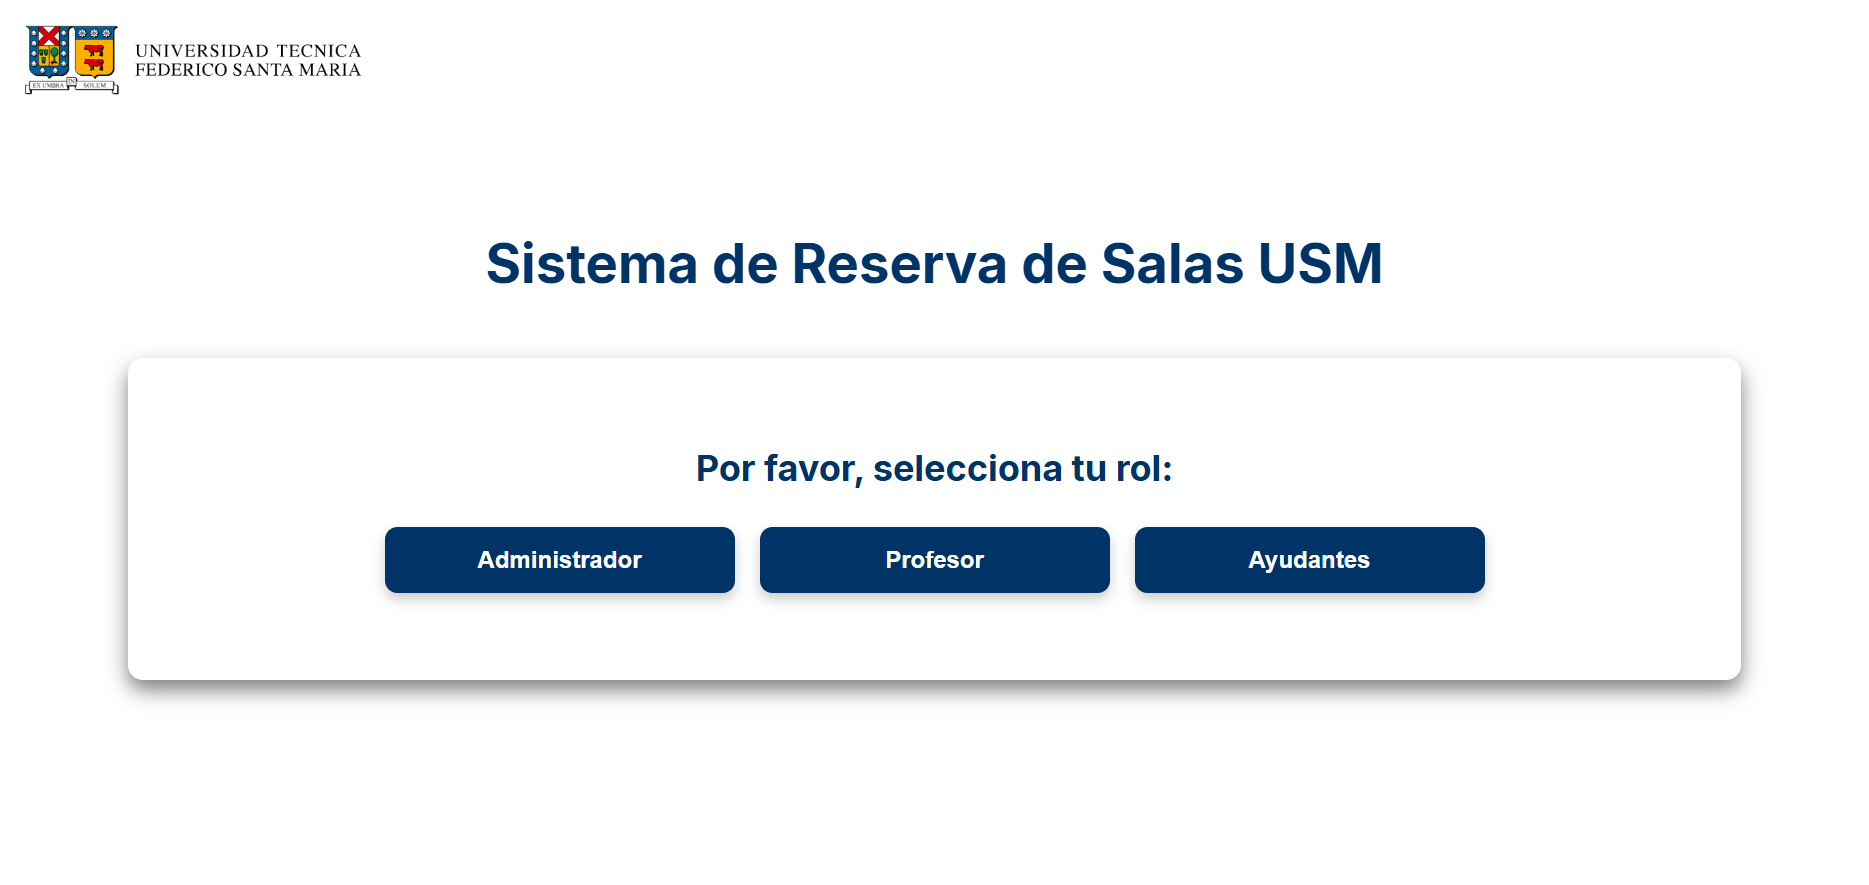
\includegraphics[width=0.8\textwidth]{IMG/ss1.png}
            \end{figure}

            \newpage
            \item \textit{Escoger salas semestrales:}
            \begin{figure}[H] 
                \centering 
                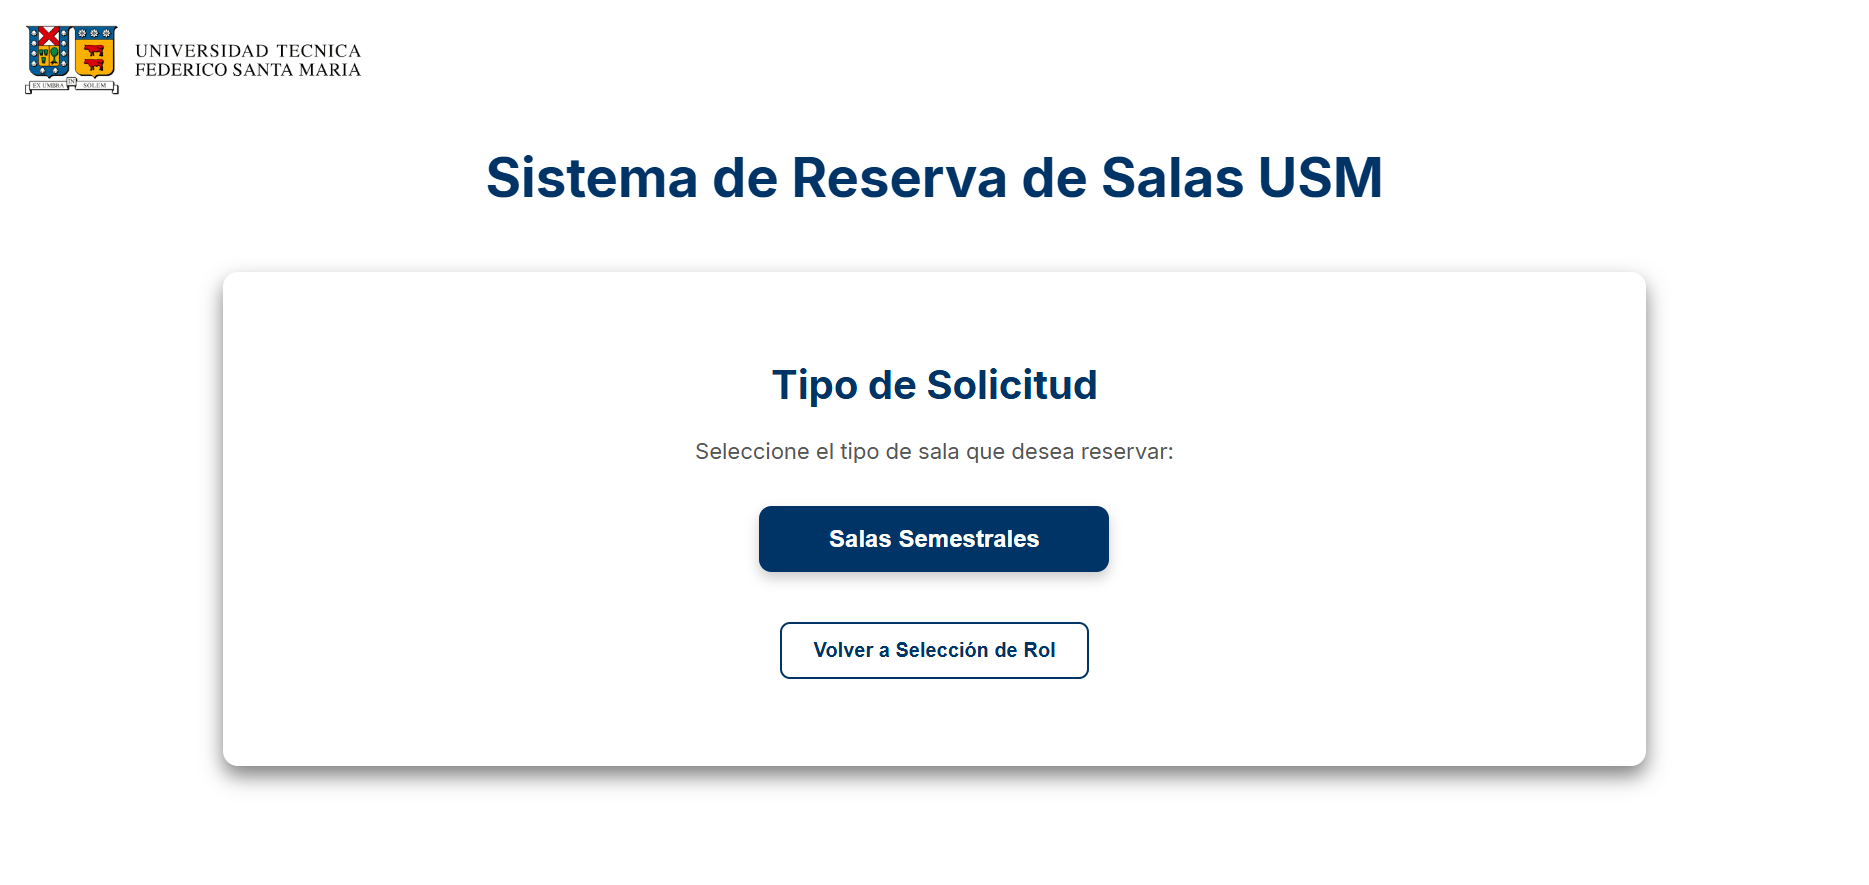
\includegraphics[width=0.8\textwidth]{IMG/ss2.png} 
            \end{figure}

            \item \textit{Escoger el Edificio B:}
            \begin{figure}[H] 
                \centering 
                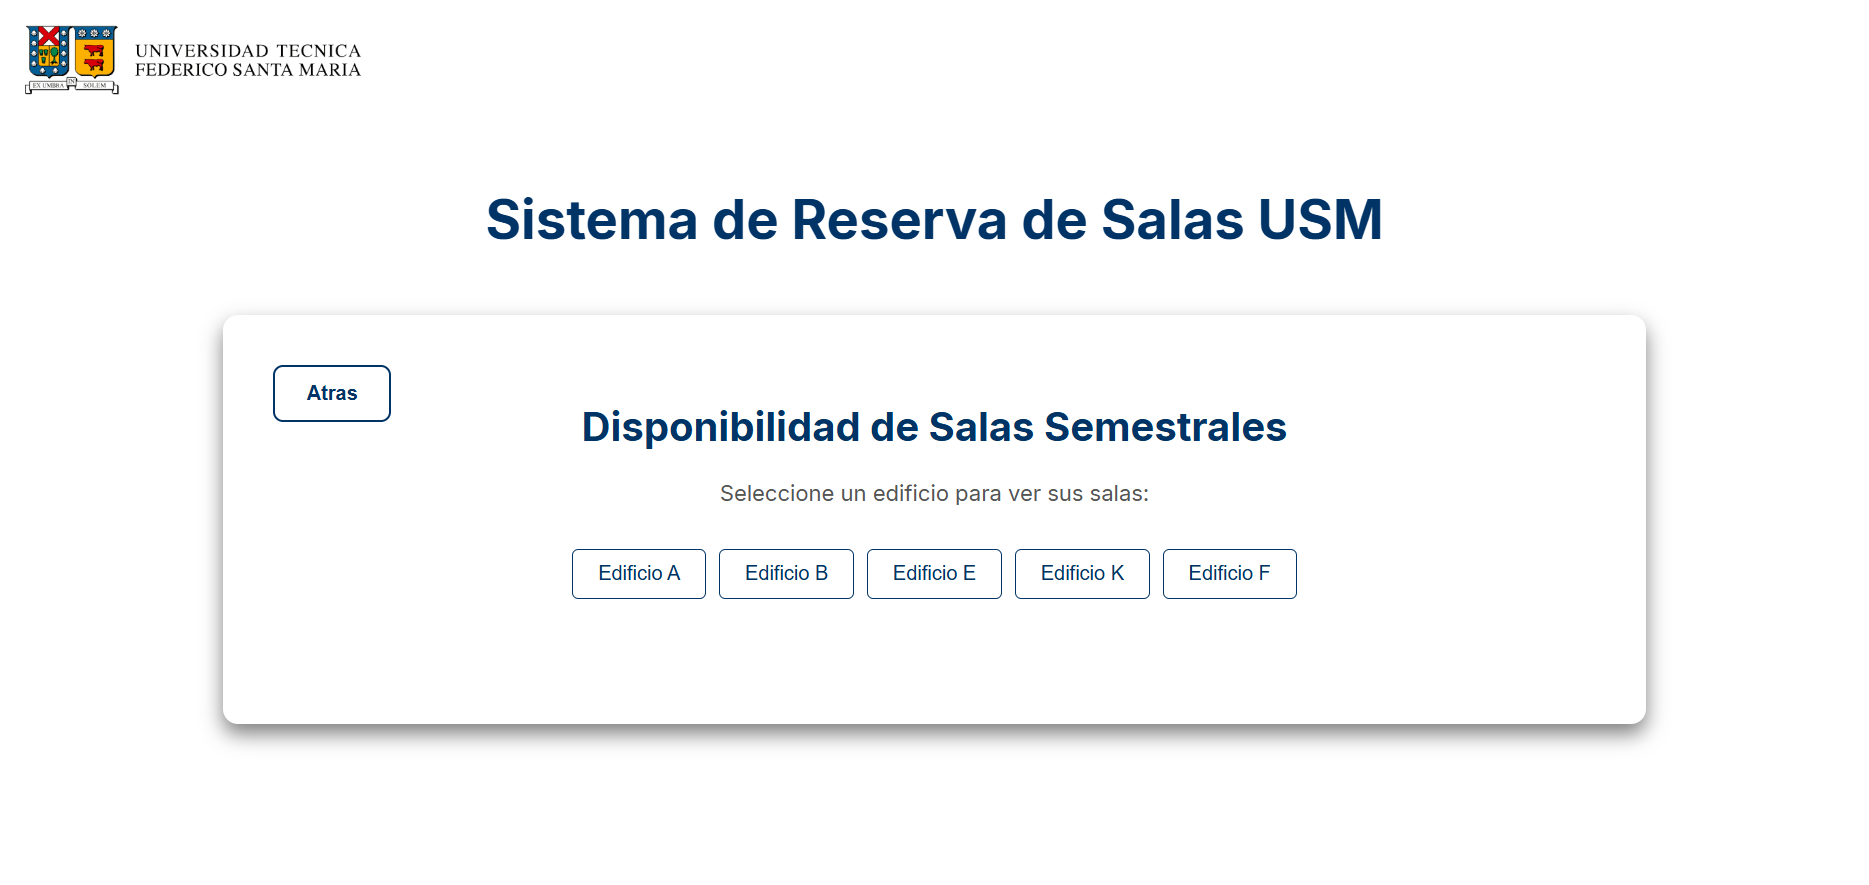
\includegraphics[width=0.8\textwidth]{IMG/ss3.png} 
            \end{figure}

            \item \textit{Ver horarios para la sala B001:}
            \begin{figure}[H] 
                \centering 
                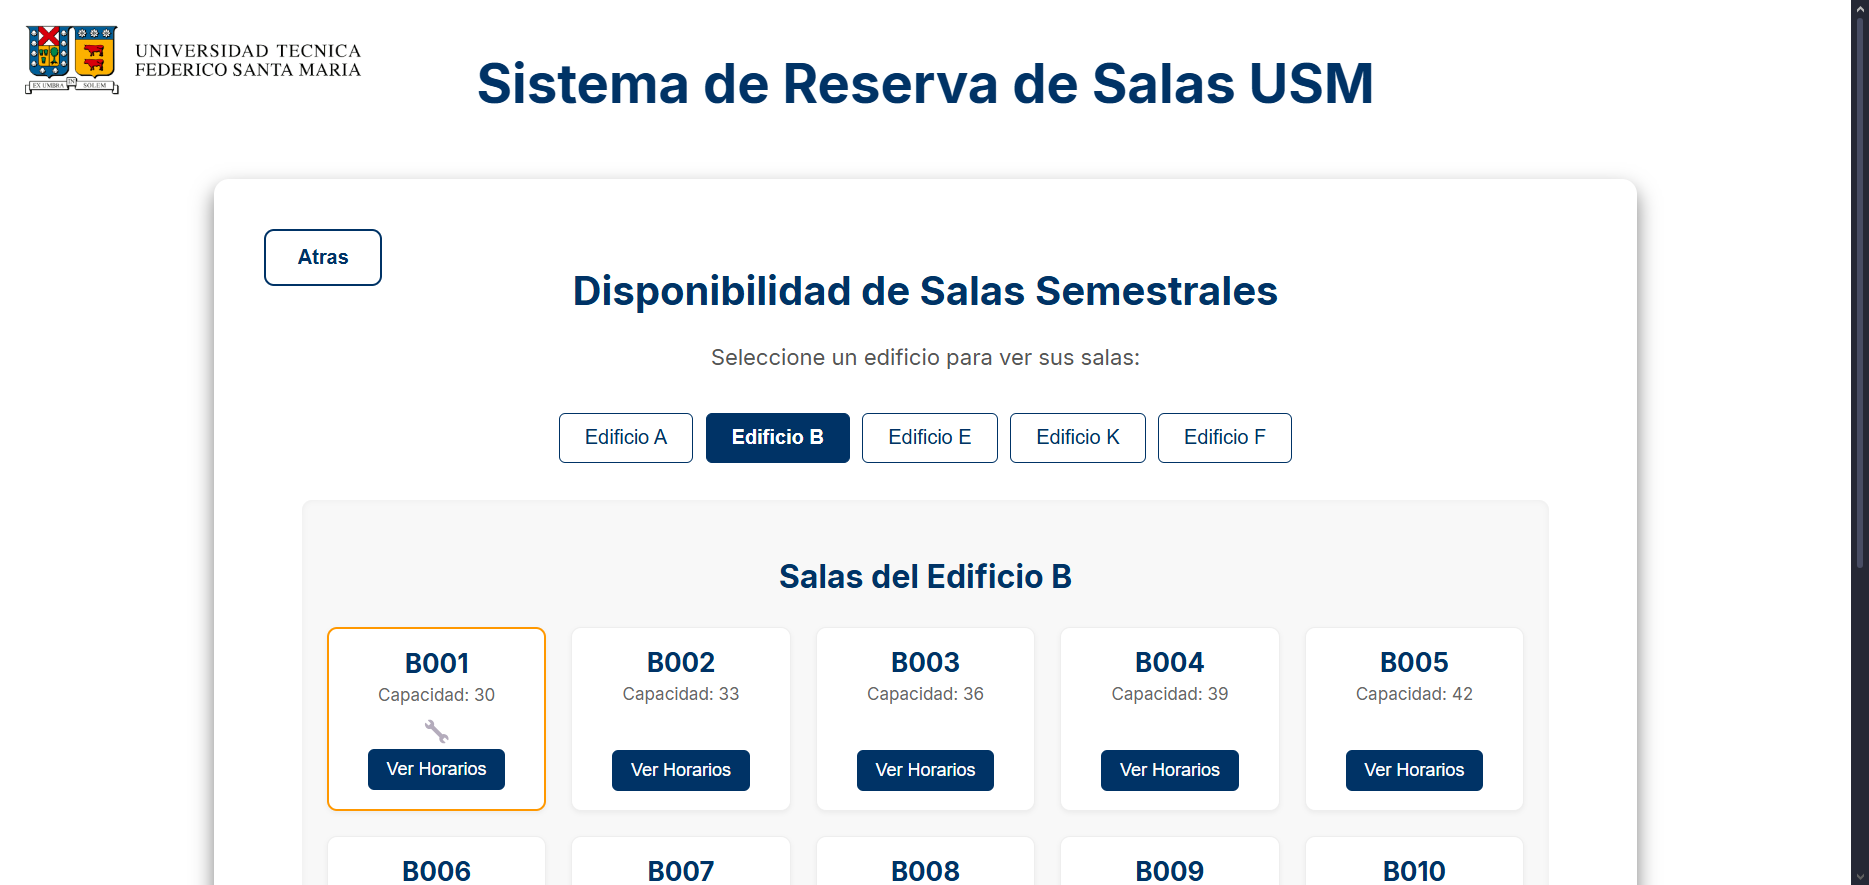
\includegraphics[width=0.8\textwidth]{IMG/ss4.png} 
            \end{figure}

            \newpage
            \item \textit{Escoger el Bloque 3-4 del dia Lunes: }
            \begin{figure}[H] 
                \centering 
                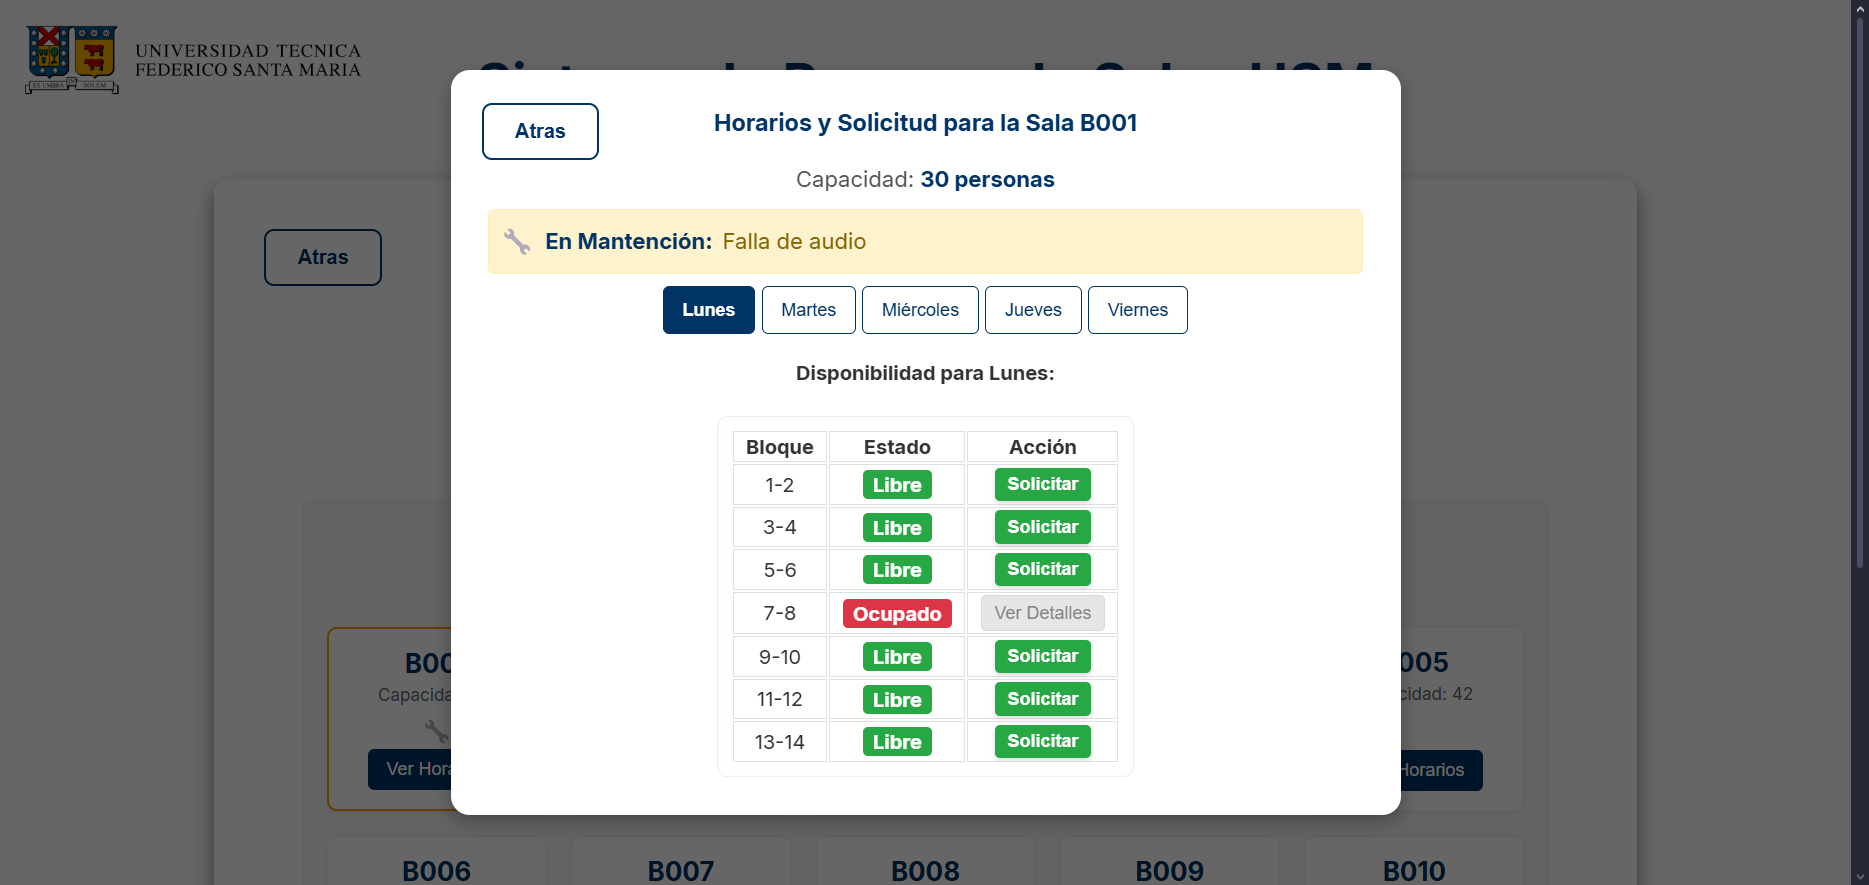
\includegraphics[width=0.8\textwidth]{IMG/ss5.png} 
            \end{figure}

            \item  \textit{Seleccionar cerrar:}
            \begin{figure}[H] 
                \centering 
                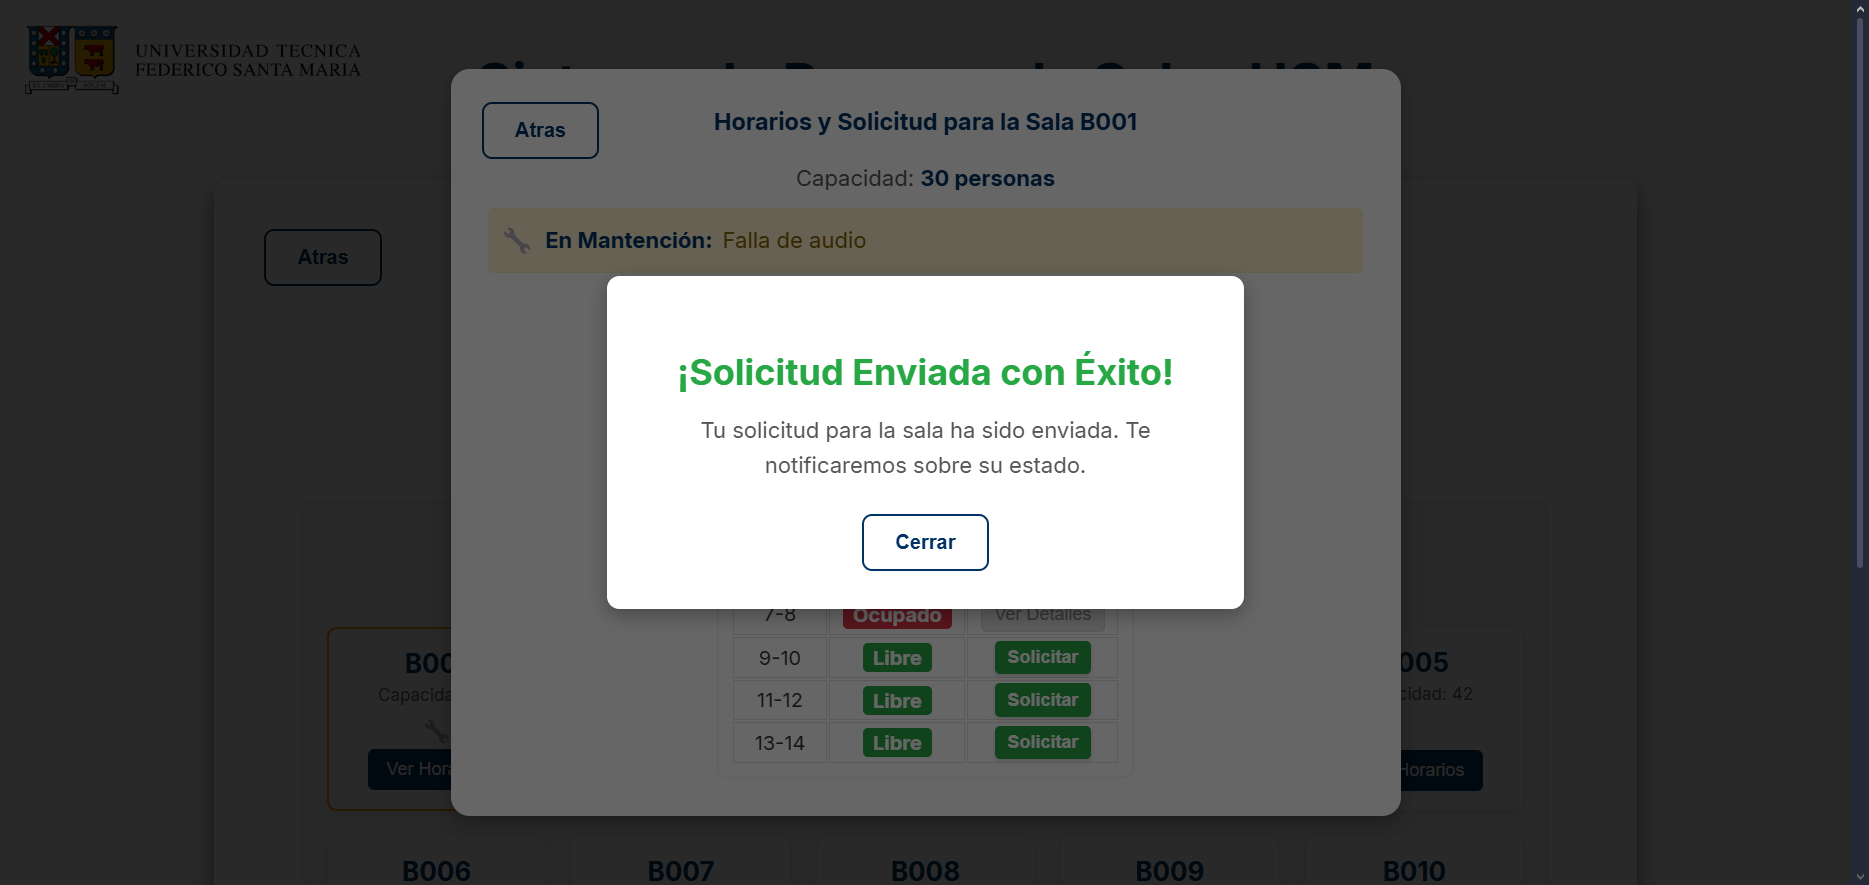
\includegraphics[width=0.8\textwidth]{IMG/ss6.png} 
            \end{figure}

            \item \textit{Estado final:}
            \begin{figure}[H] 
                \centering 
                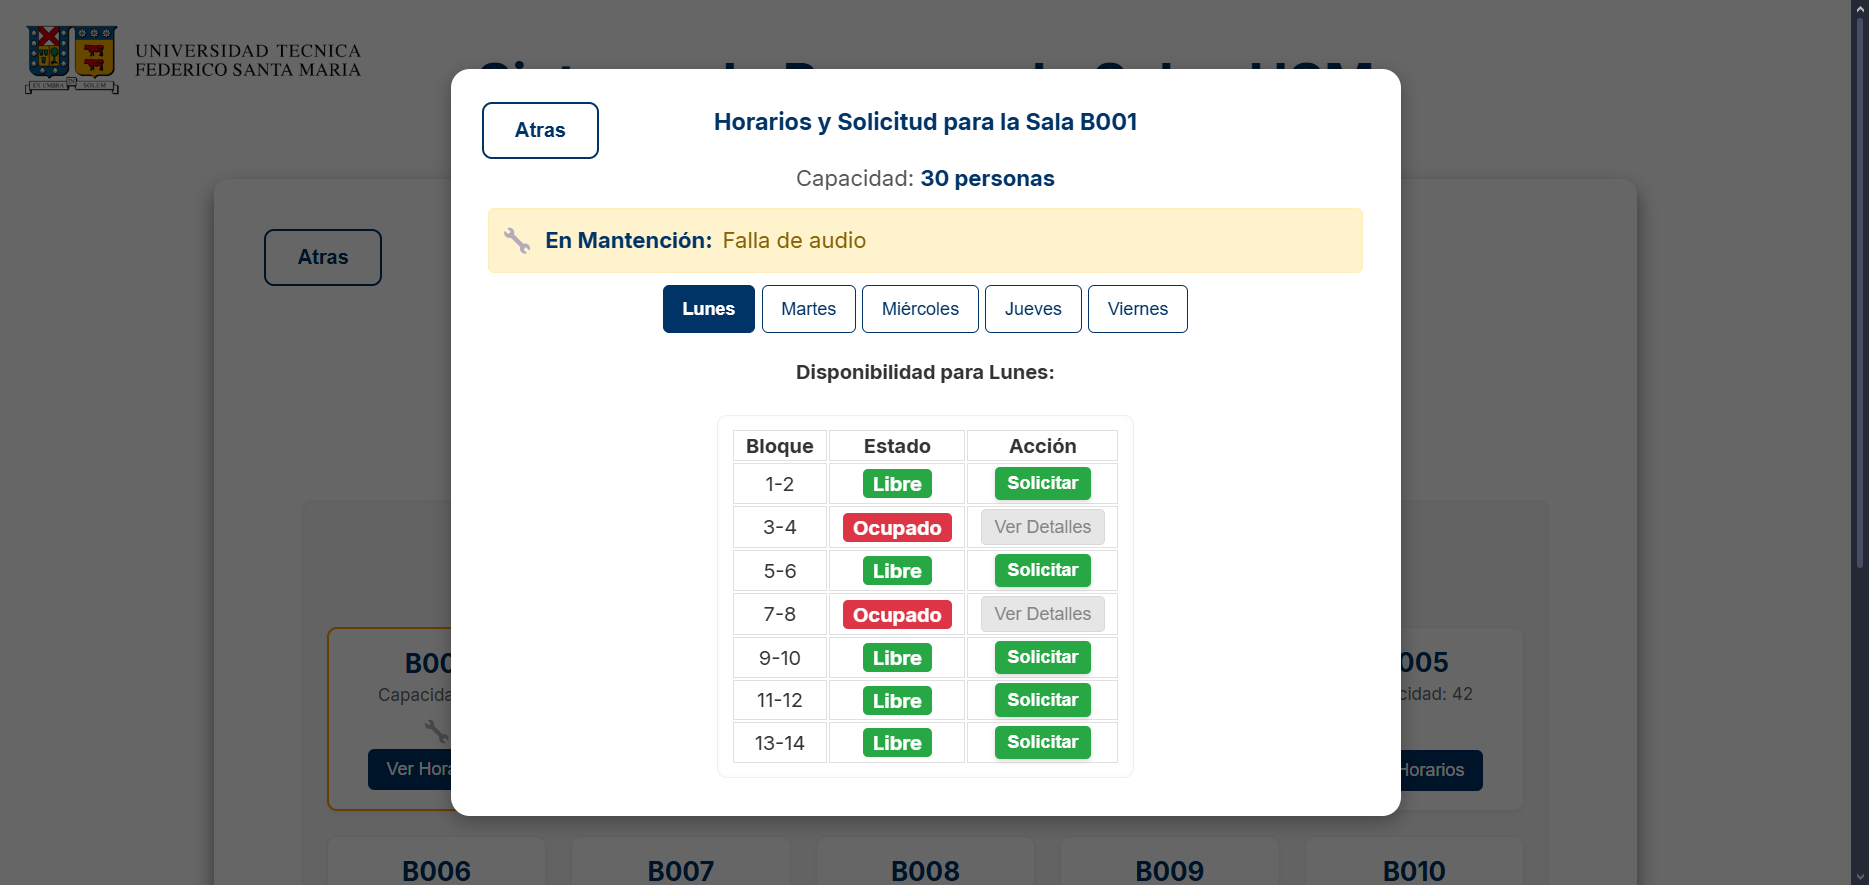
\includegraphics[width=0.8\textwidth]{IMG/ss7.png} 
            \end{figure}
        \end{enumerate}
        \newpage
        
        
        \item \textbf{Solicitar sala semestral Profesor:}
        \begin{enumerate}
            \item \textit{Escoger rol profesor:}
            \begin{figure}[H] 
                \centering 
                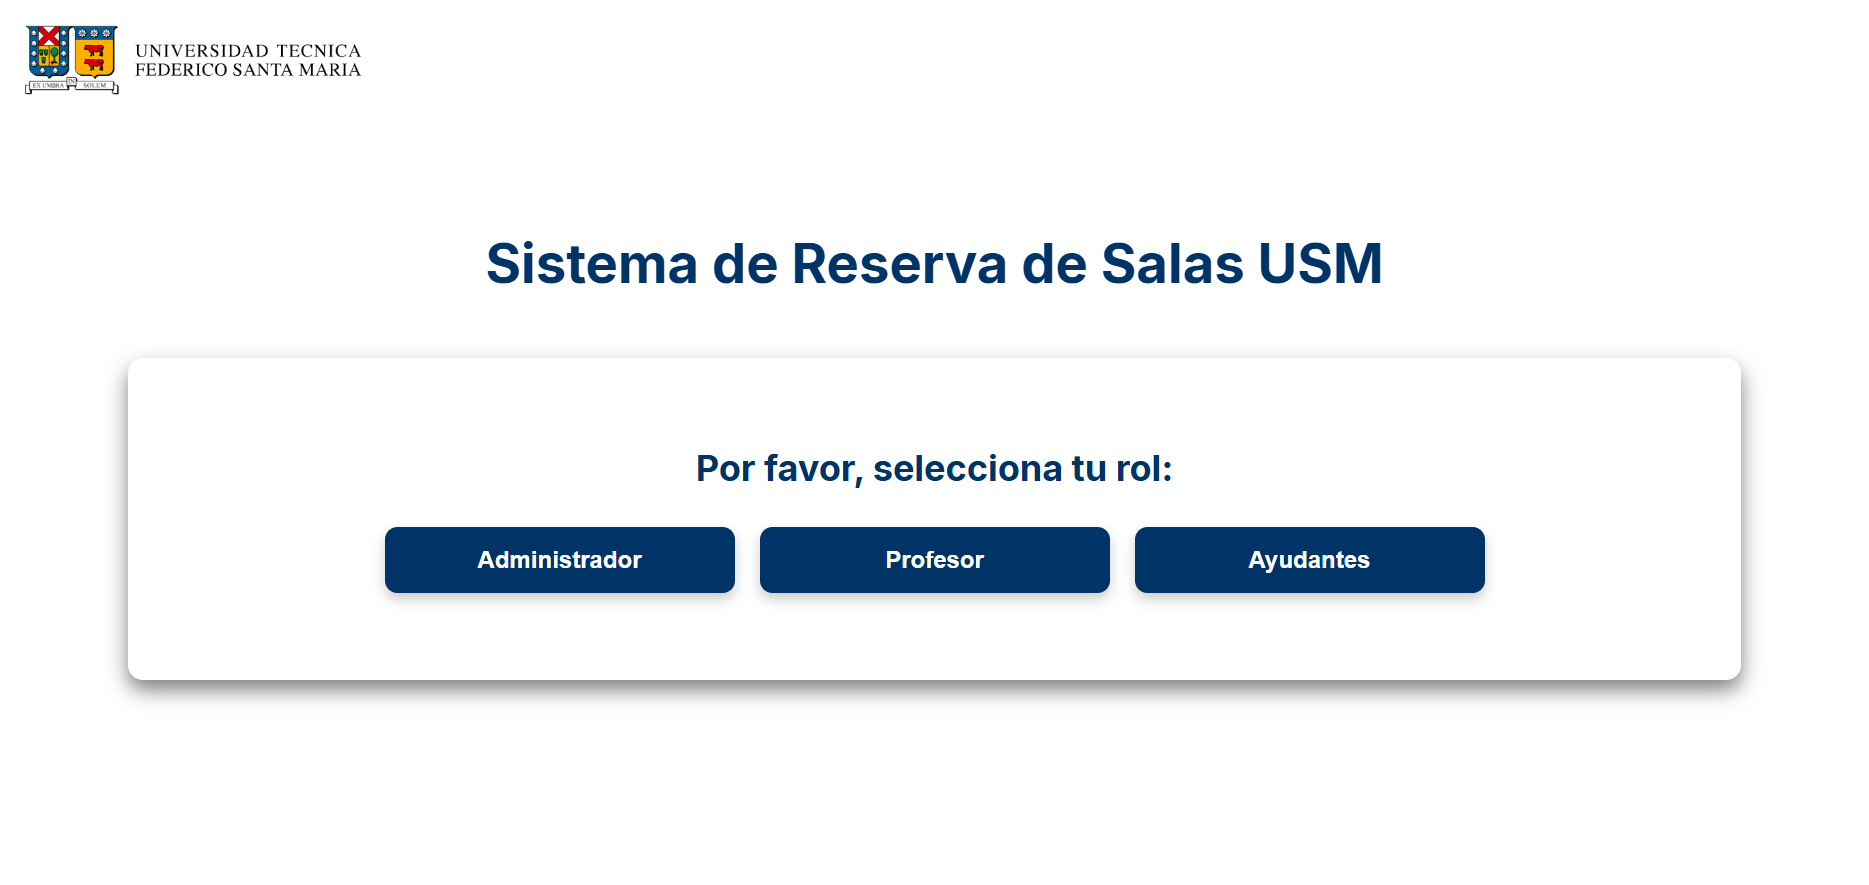
\includegraphics[width=0.8\textwidth]{IMG/ss1.png} 
            \end{figure}

            \item \textit{Escoger salas semestrales:}
            \begin{figure}[H] 
                \centering 
                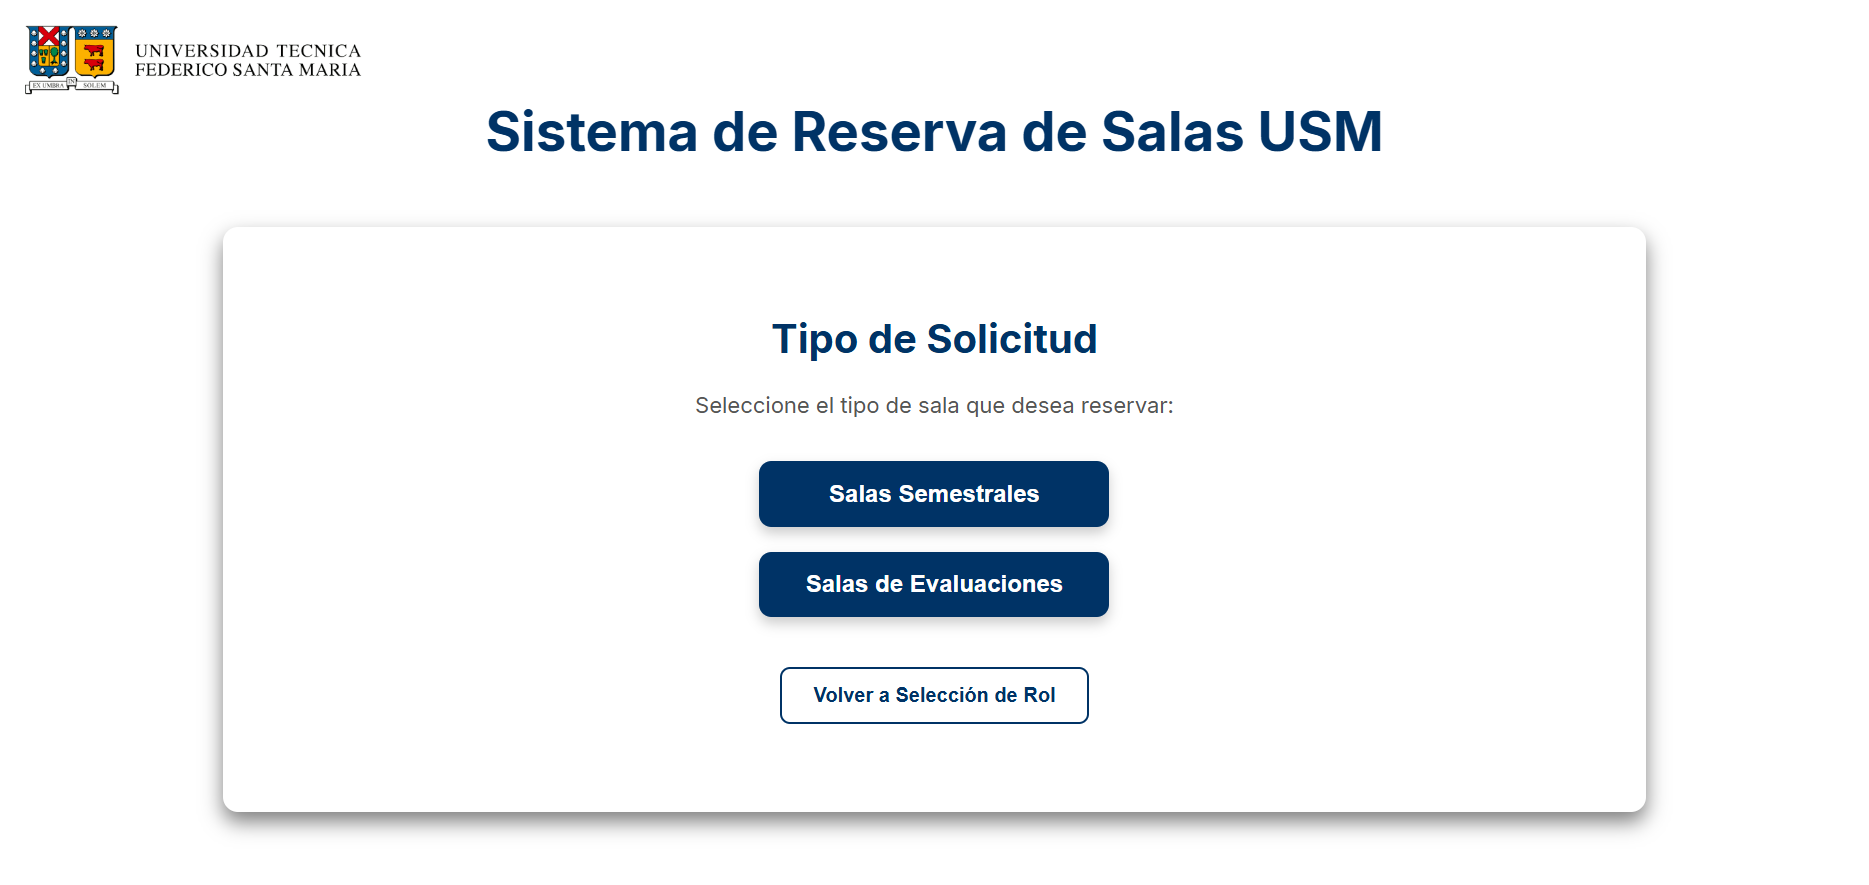
\includegraphics[width=0.8\textwidth]{IMG/ss9.png} 
            \end{figure}

            \item \textit{Escoger el Edificio A:}
            \begin{figure}[H] 
                \centering 
                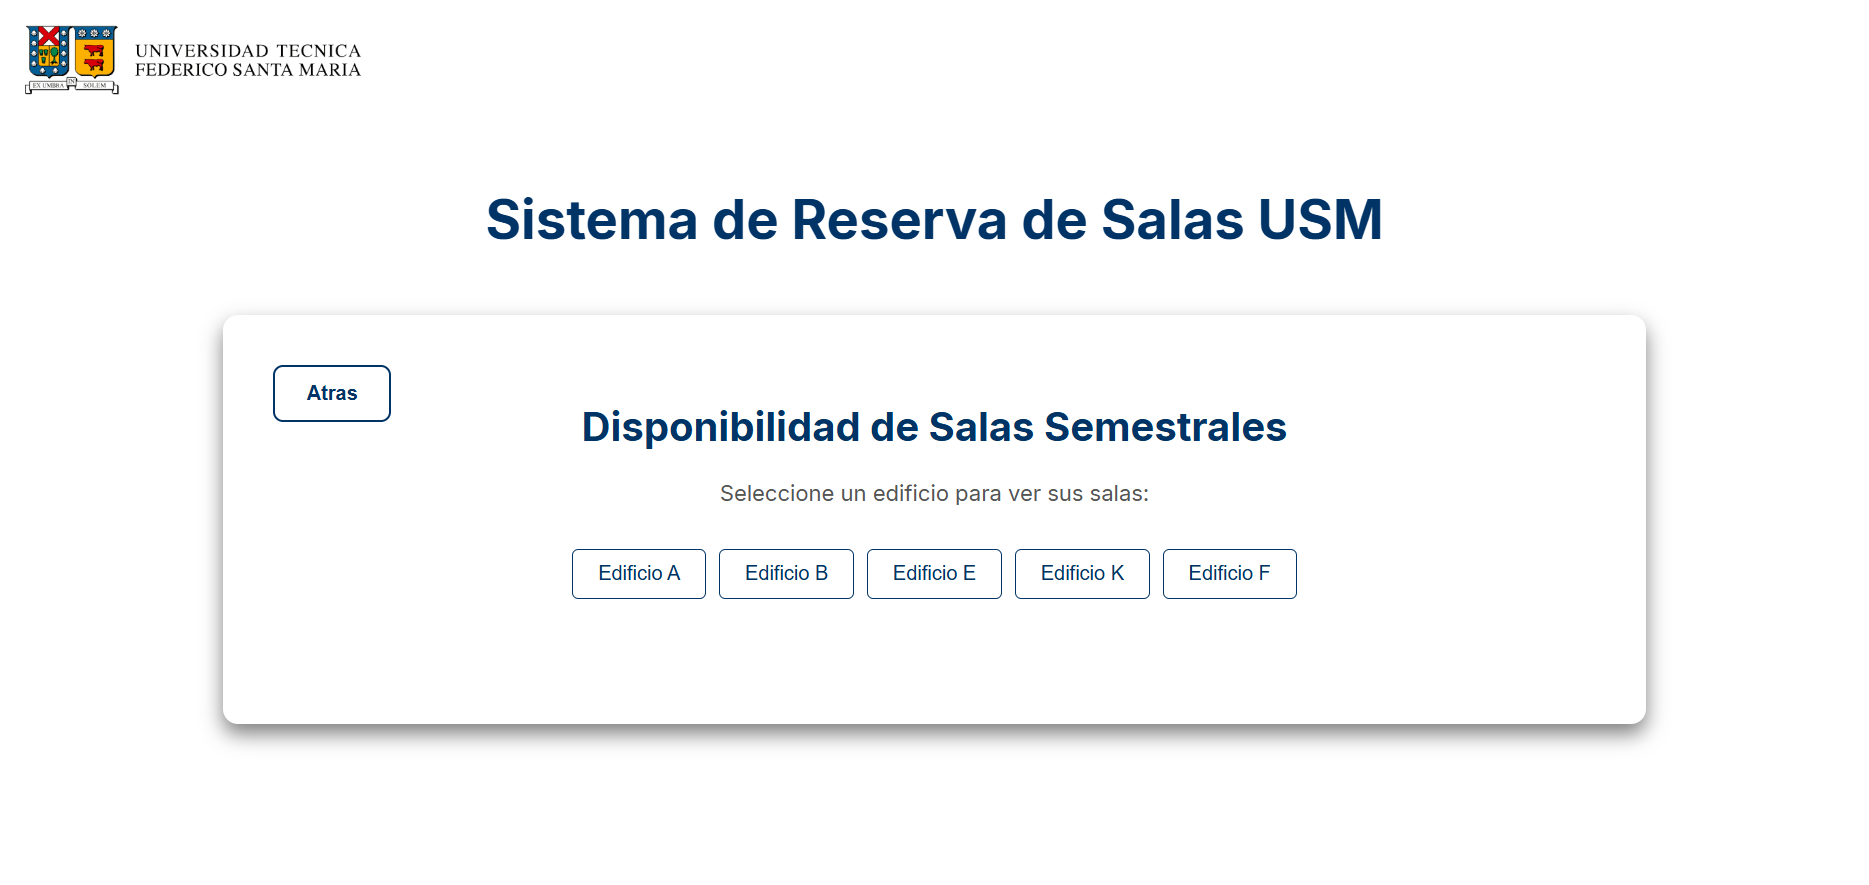
\includegraphics[width=0.8\textwidth]{IMG/ss10.png} 
            \end{figure}

            \newpage
            \item \textit{Ver horarios para la sala A001:}
            \begin{figure}[H] 
                \centering 
                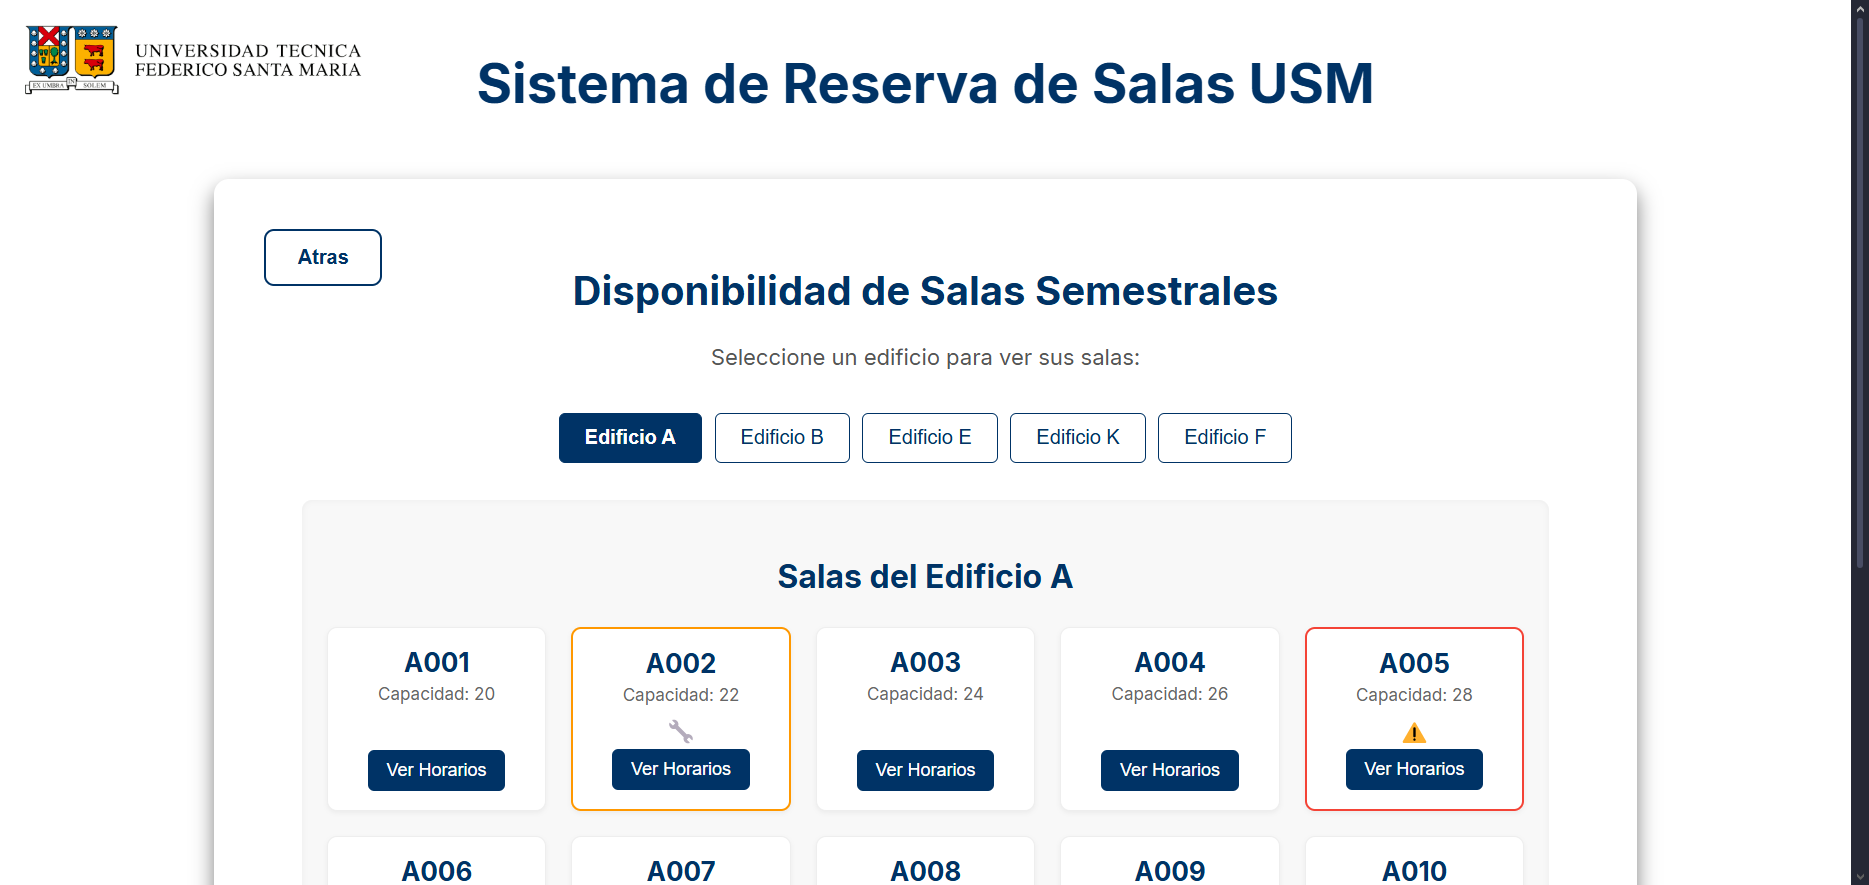
\includegraphics[width=0.8\textwidth]{IMG/ss11.png} 
            \end{figure}

            \item  \textit{Escoger el Bloque 11-12 el dia Lunes:}
            \begin{figure}[H] 
                \centering 
                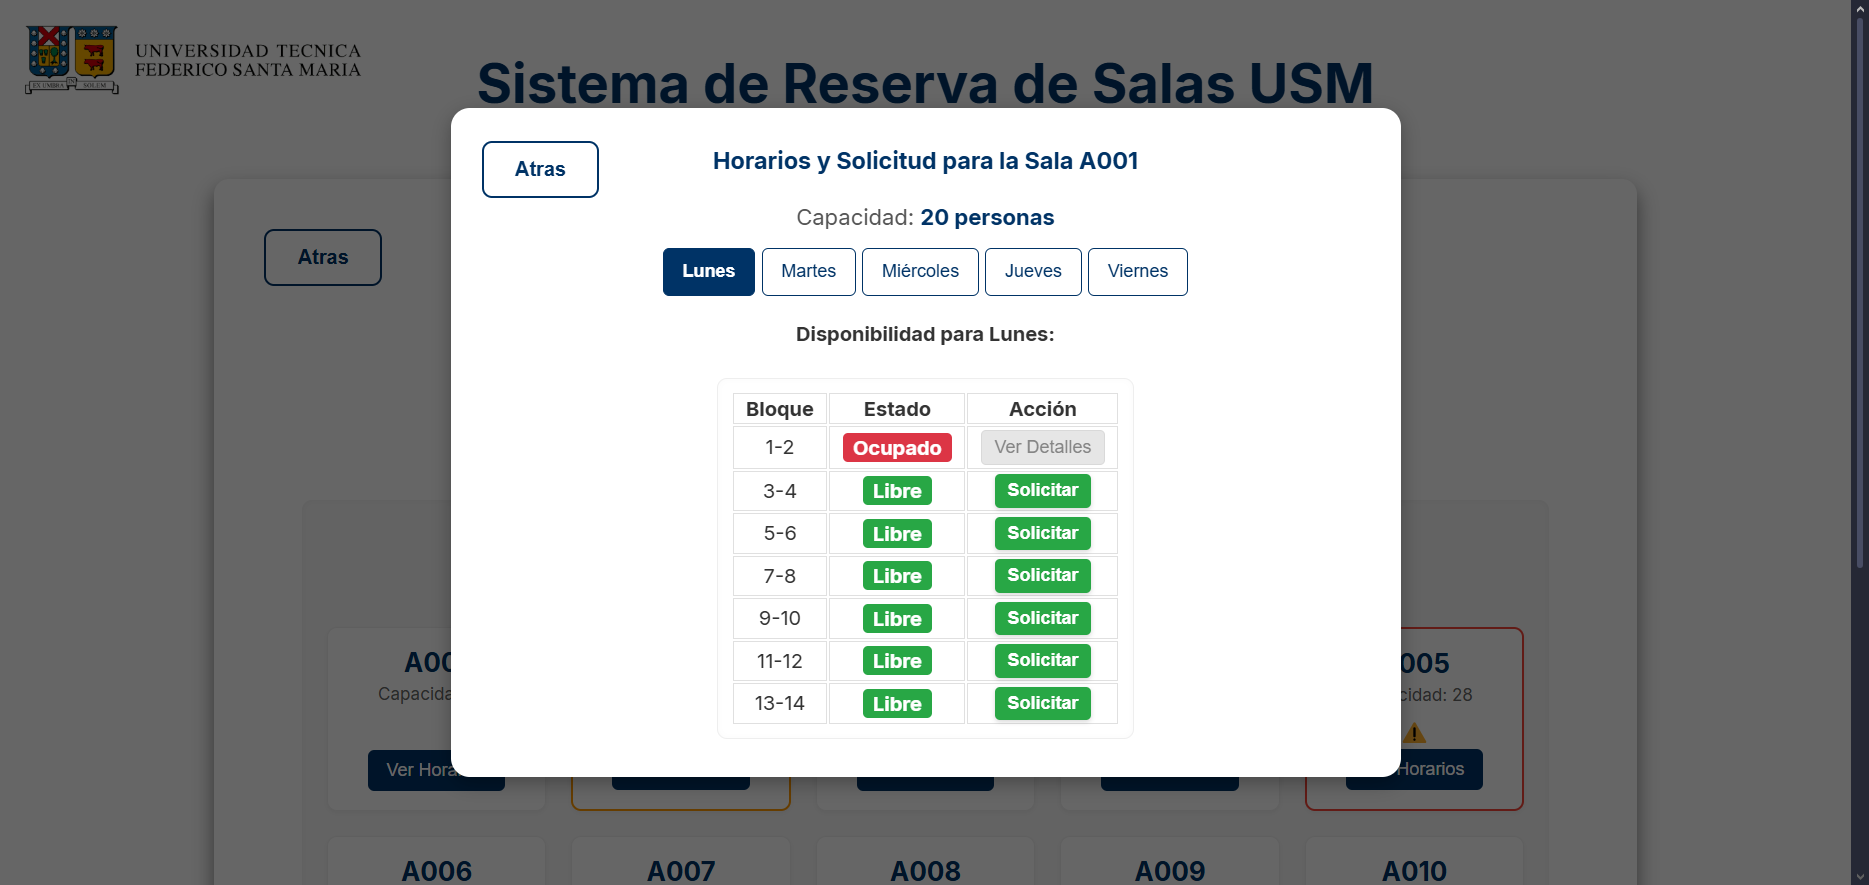
\includegraphics[width=0.8\textwidth]{IMG/ss12.png} 
            \end{figure}

            \item \textit{Seleccionar cerrar:}
            \begin{figure}[H] 
                \centering 
                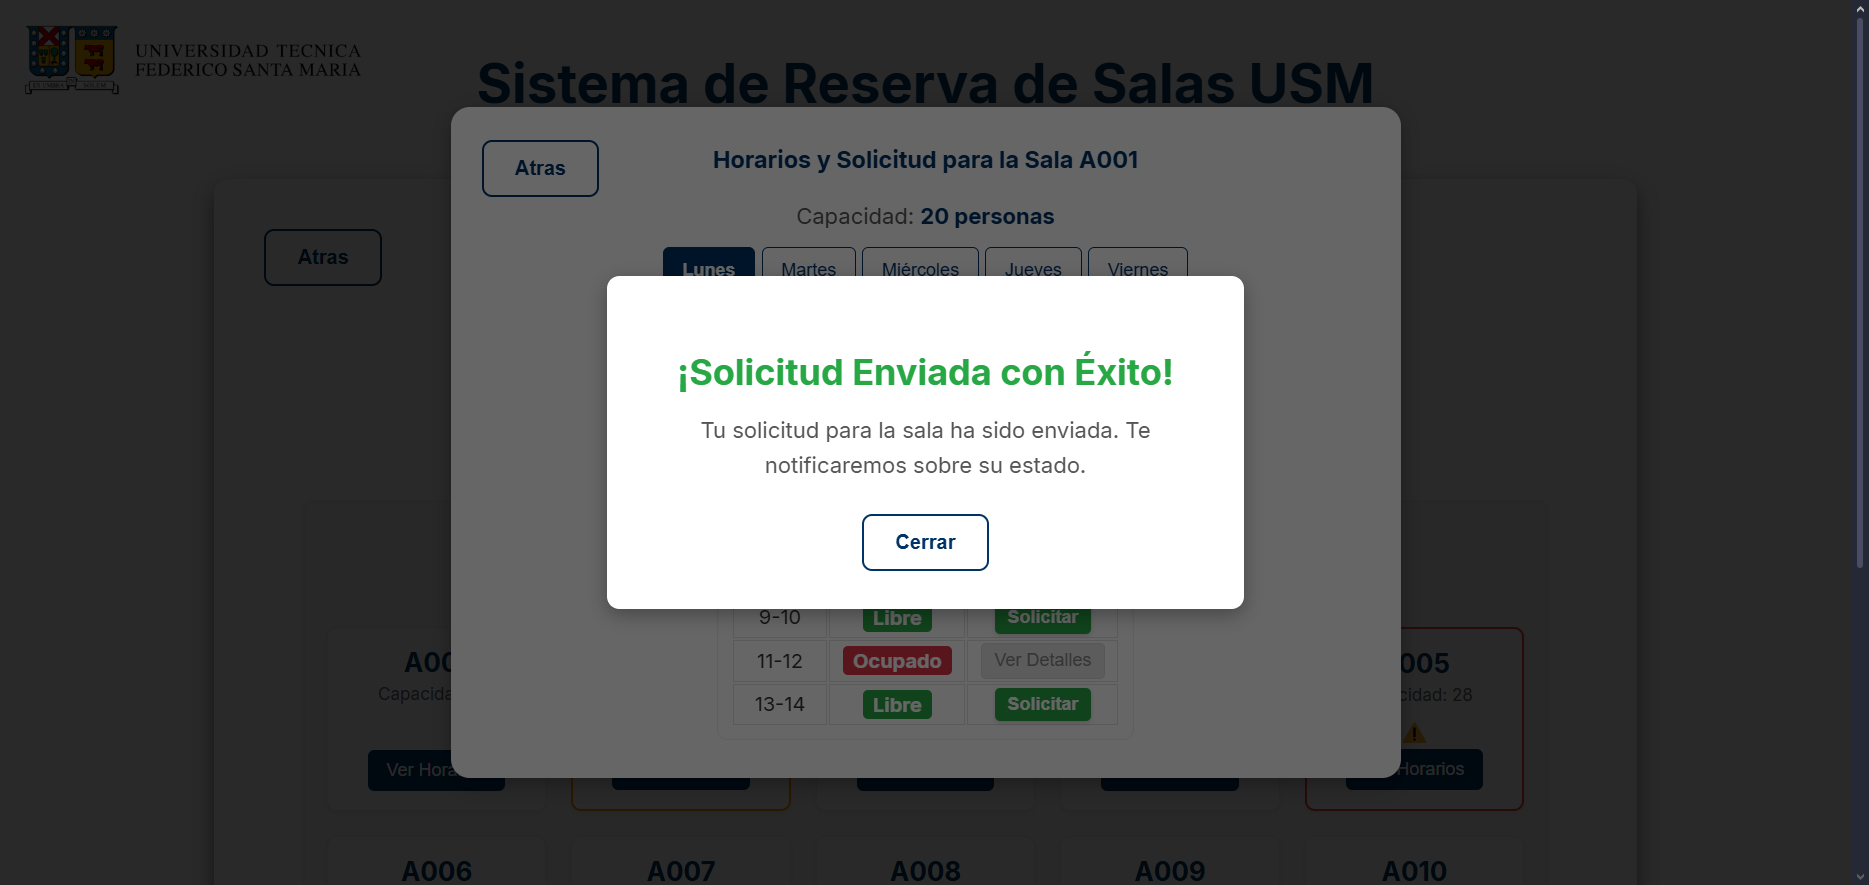
\includegraphics[width=0.8\textwidth]{IMG/ss13.png}
            \end{figure}
            
            \newpage
            \item  \textit{Estado final:}
            \begin{figure}[H] 
                \centering 
                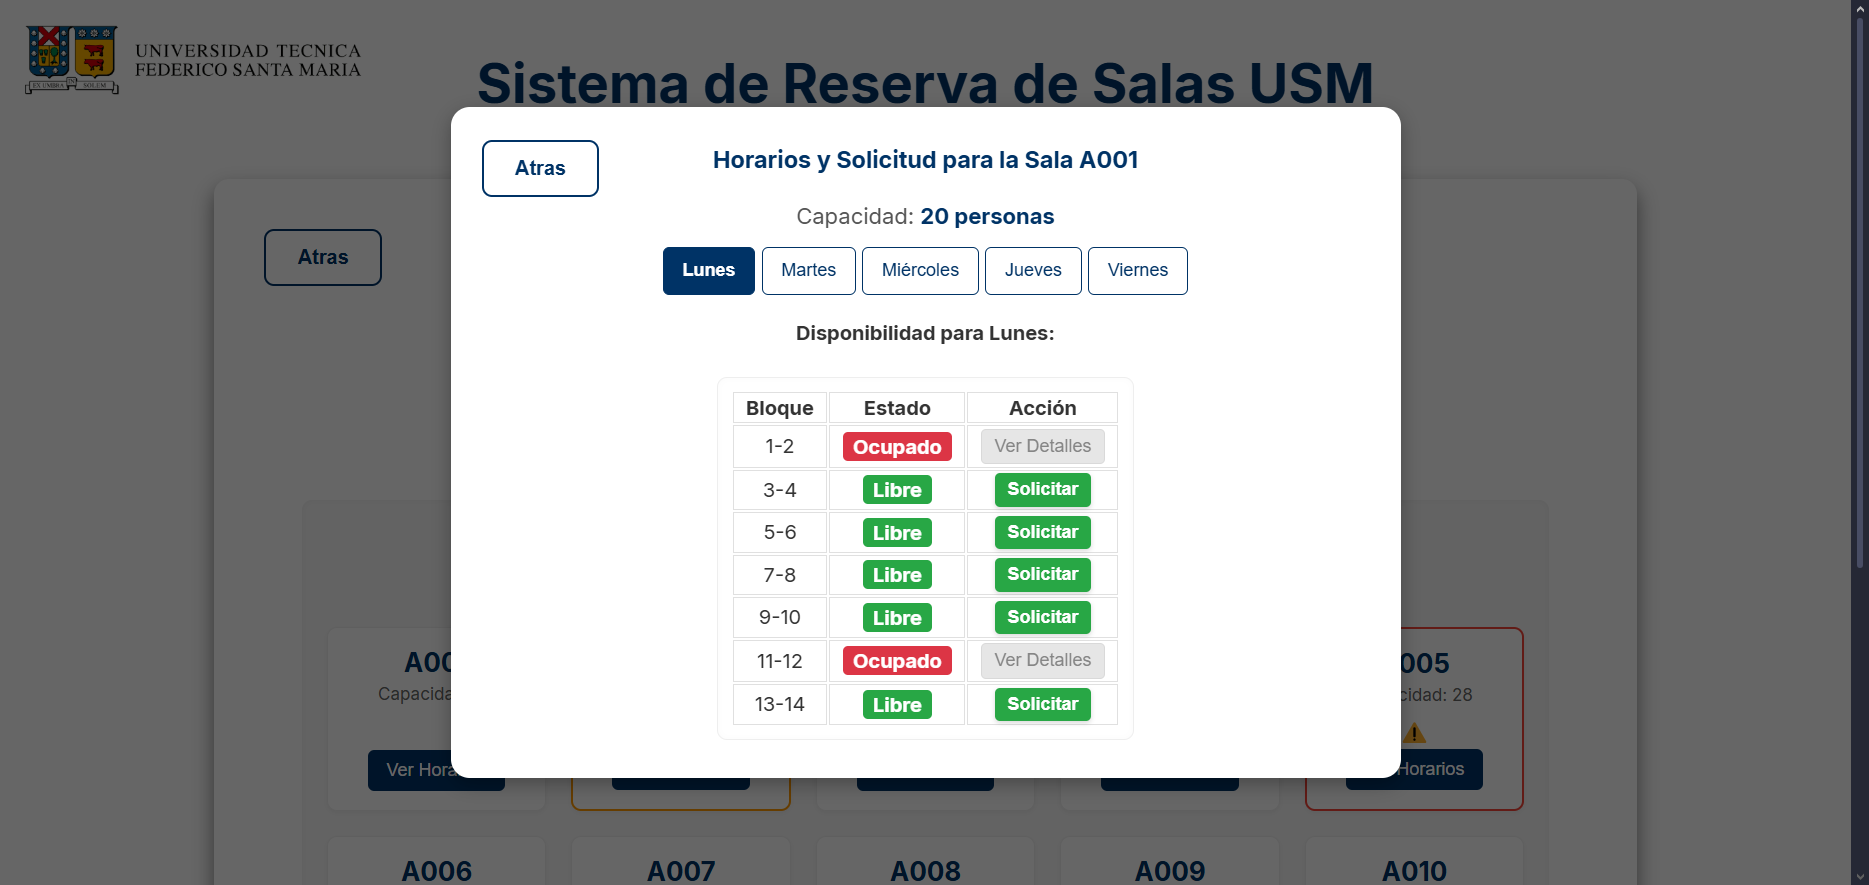
\includegraphics[width=0.8\textwidth]{IMG/ss14.png} 
            \end{figure}
        \end{enumerate}
        
        
        \item \textbf{Solicitar sala para evaluación Profesor:}
        \begin{enumerate}
            \item \textit{Escoger rol profesor:}
            \begin{figure}[H] 
                \centering 
                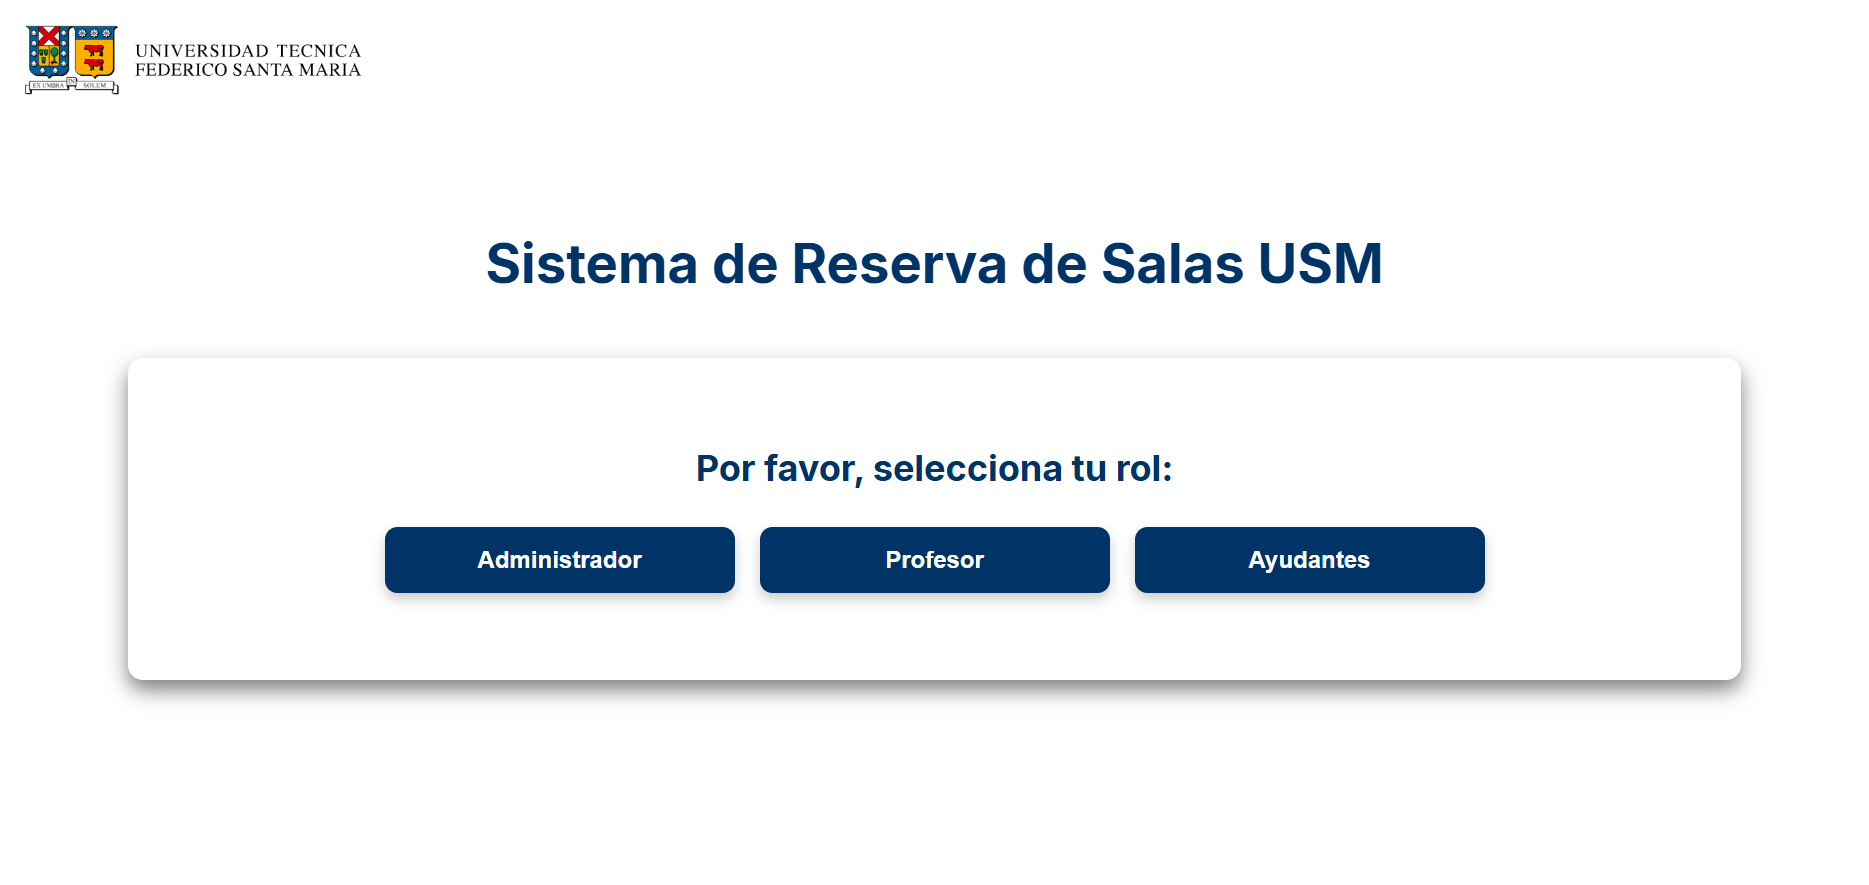
\includegraphics[width=0.8\textwidth]{IMG/ss1.png} 
            \end{figure}

            \item \textit{Escoger salas de evaluaciones:}
            \begin{figure}[H] 
                \centering 
                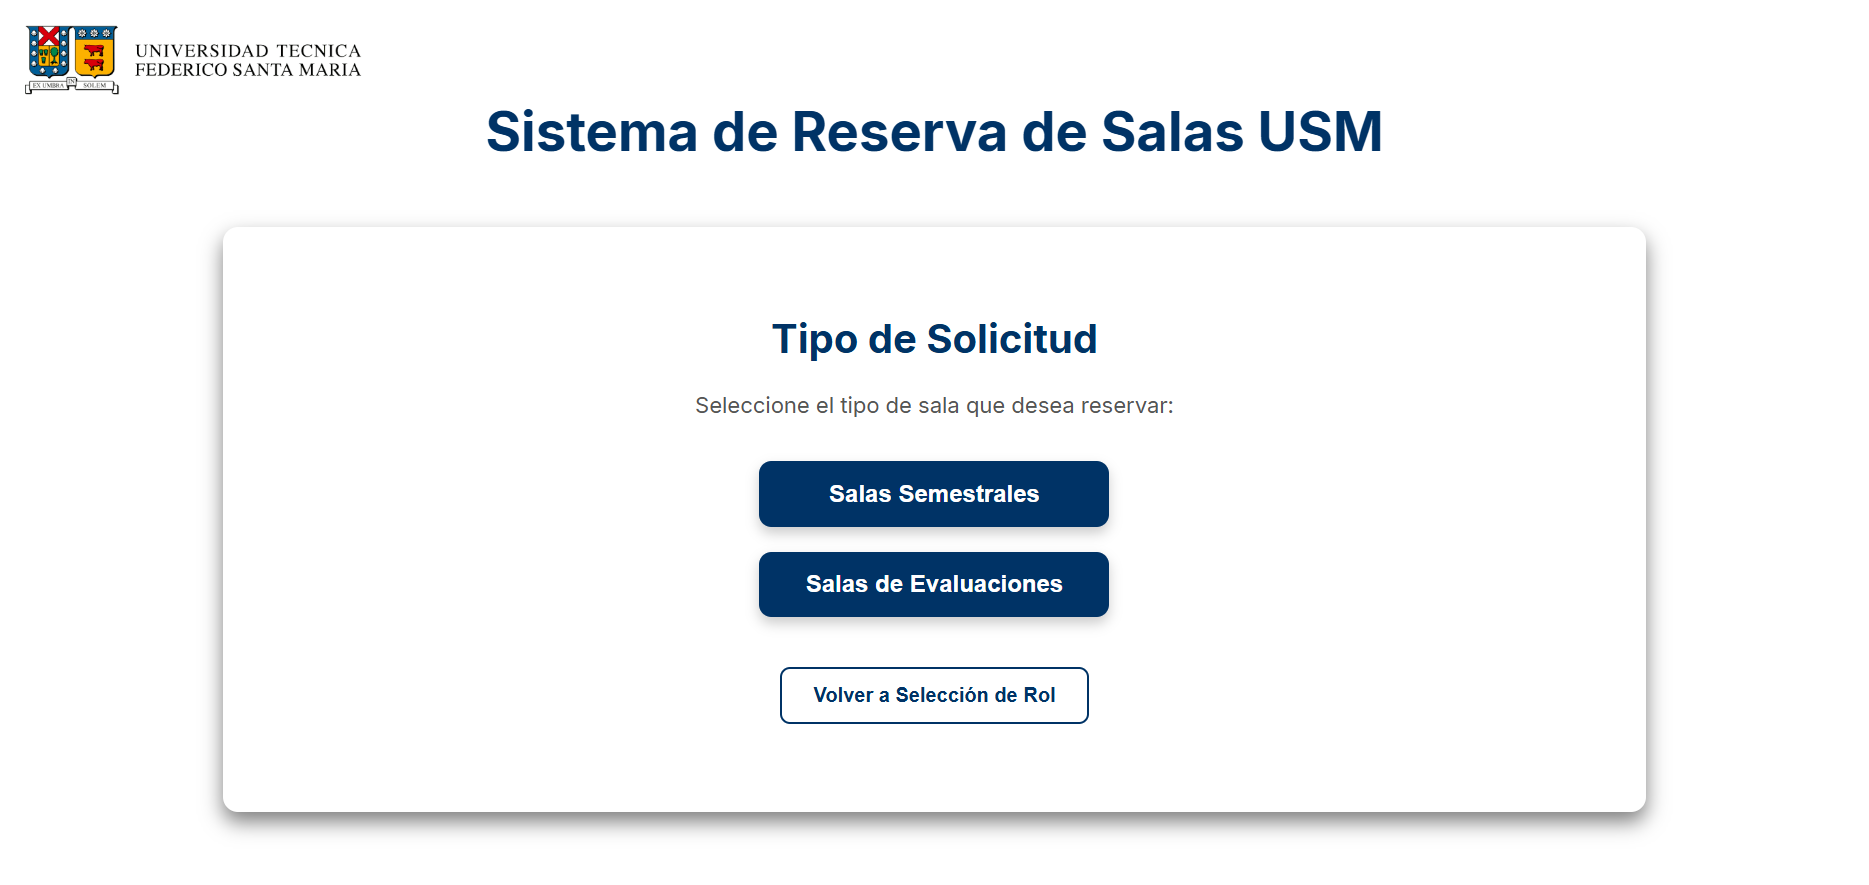
\includegraphics[width=0.8\textwidth]{IMG/ss9.png} 
            \end{figure}

            \newpage
            \item \textit{Seleccionar fecha:}
            \begin{figure}[H] 
                \centering 
                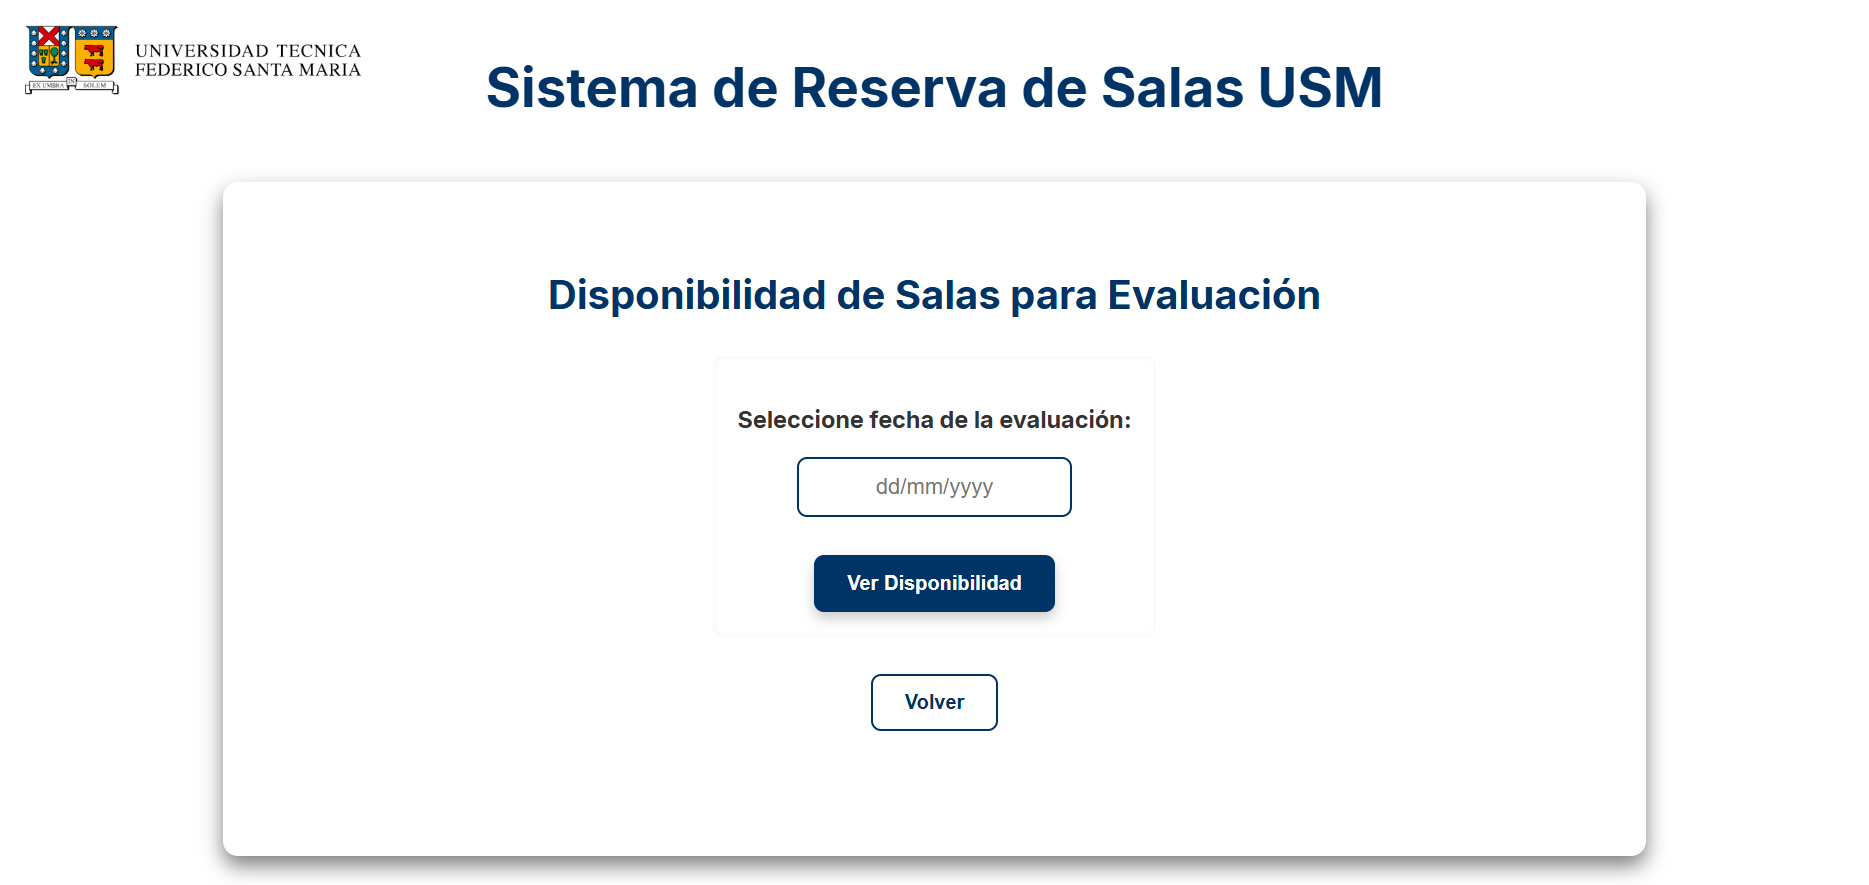
\includegraphics[width=0.8\textwidth]{IMG/ss15.png} 
            \end{figure}

            
            \item \textit{Escoger 10 de Junio:}
            \begin{figure}[H] 
                \centering 
                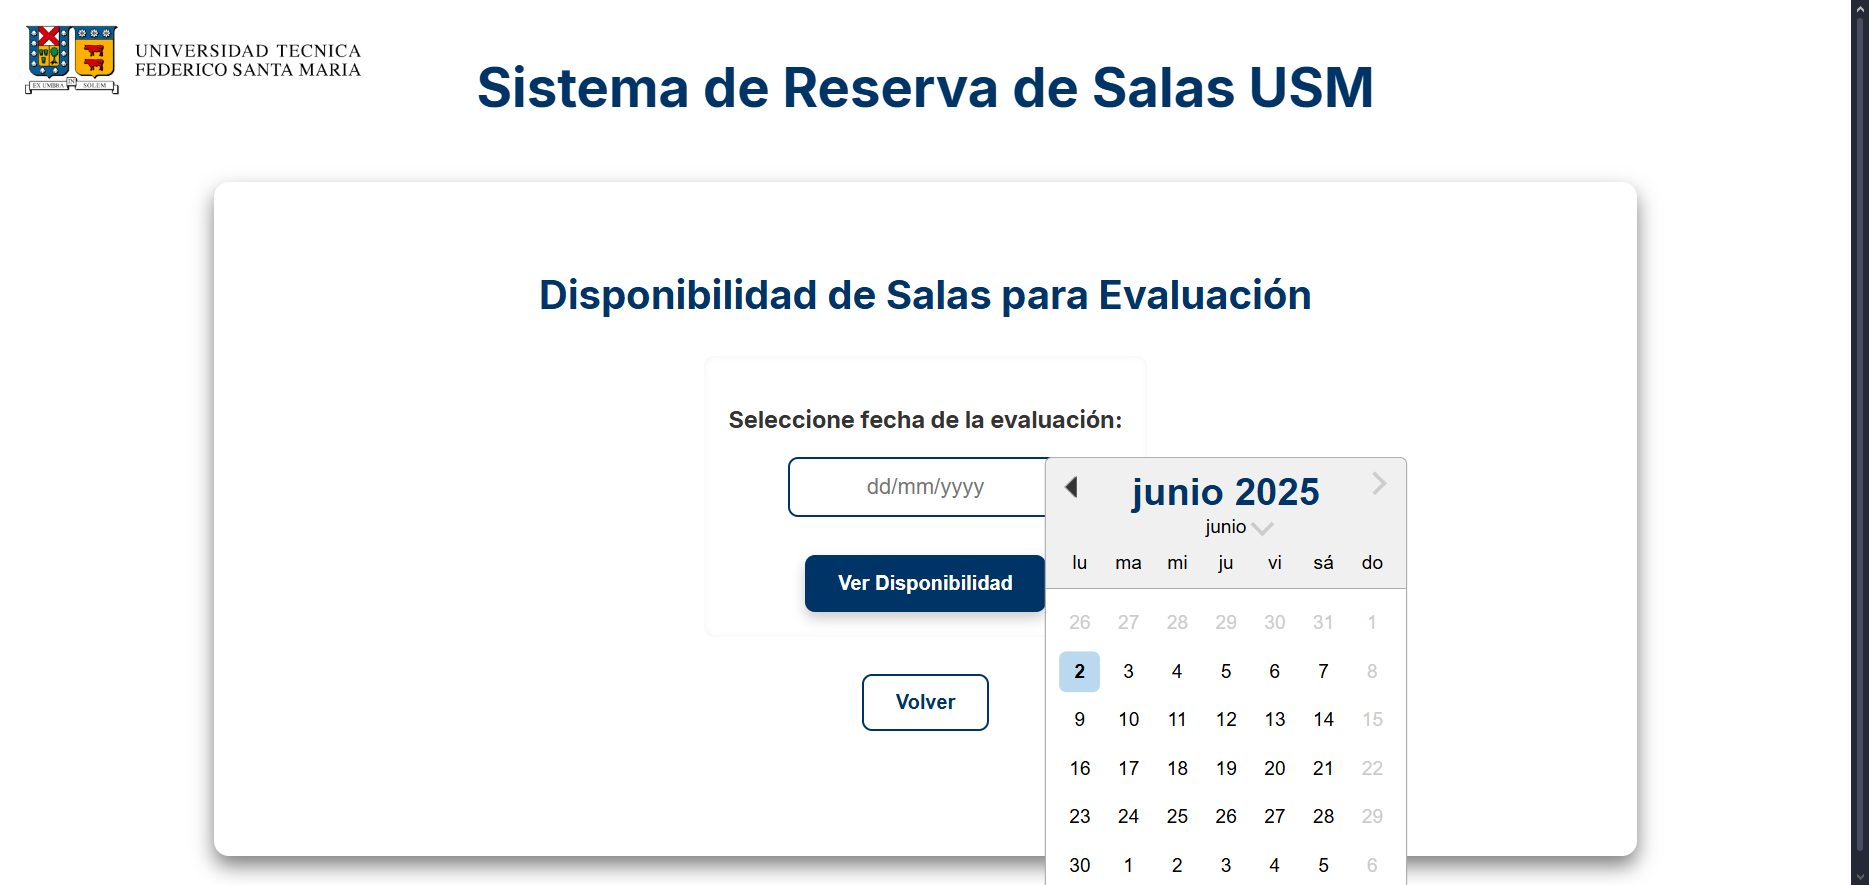
\includegraphics[width=0.8\textwidth]{IMG/ss16.png} 
            \end{figure}

            \item  \textit{Pinchar Ver Disponibilidad:}
            \begin{figure}[H] 
                \centering 
                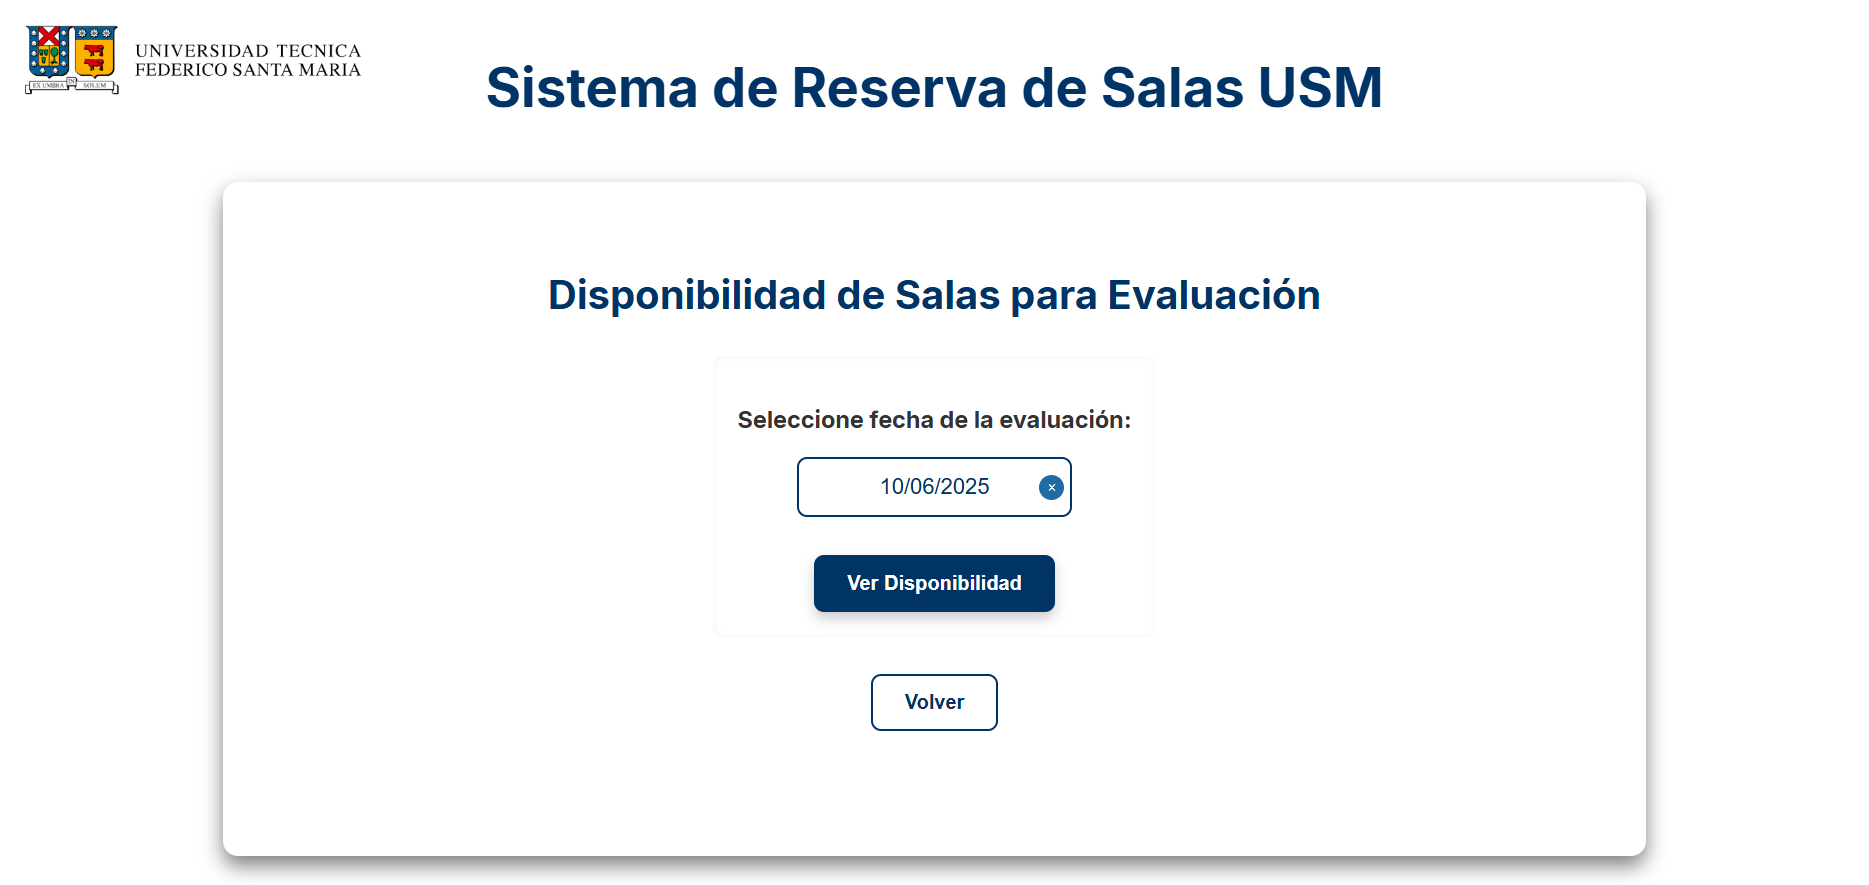
\includegraphics[width=0.8\textwidth]{IMG/ss17.png} 
            \end{figure}
            
            \newpage
            \item \textit{Escoger el Edificio K:}
            \begin{figure}[H] 
                \centering 
                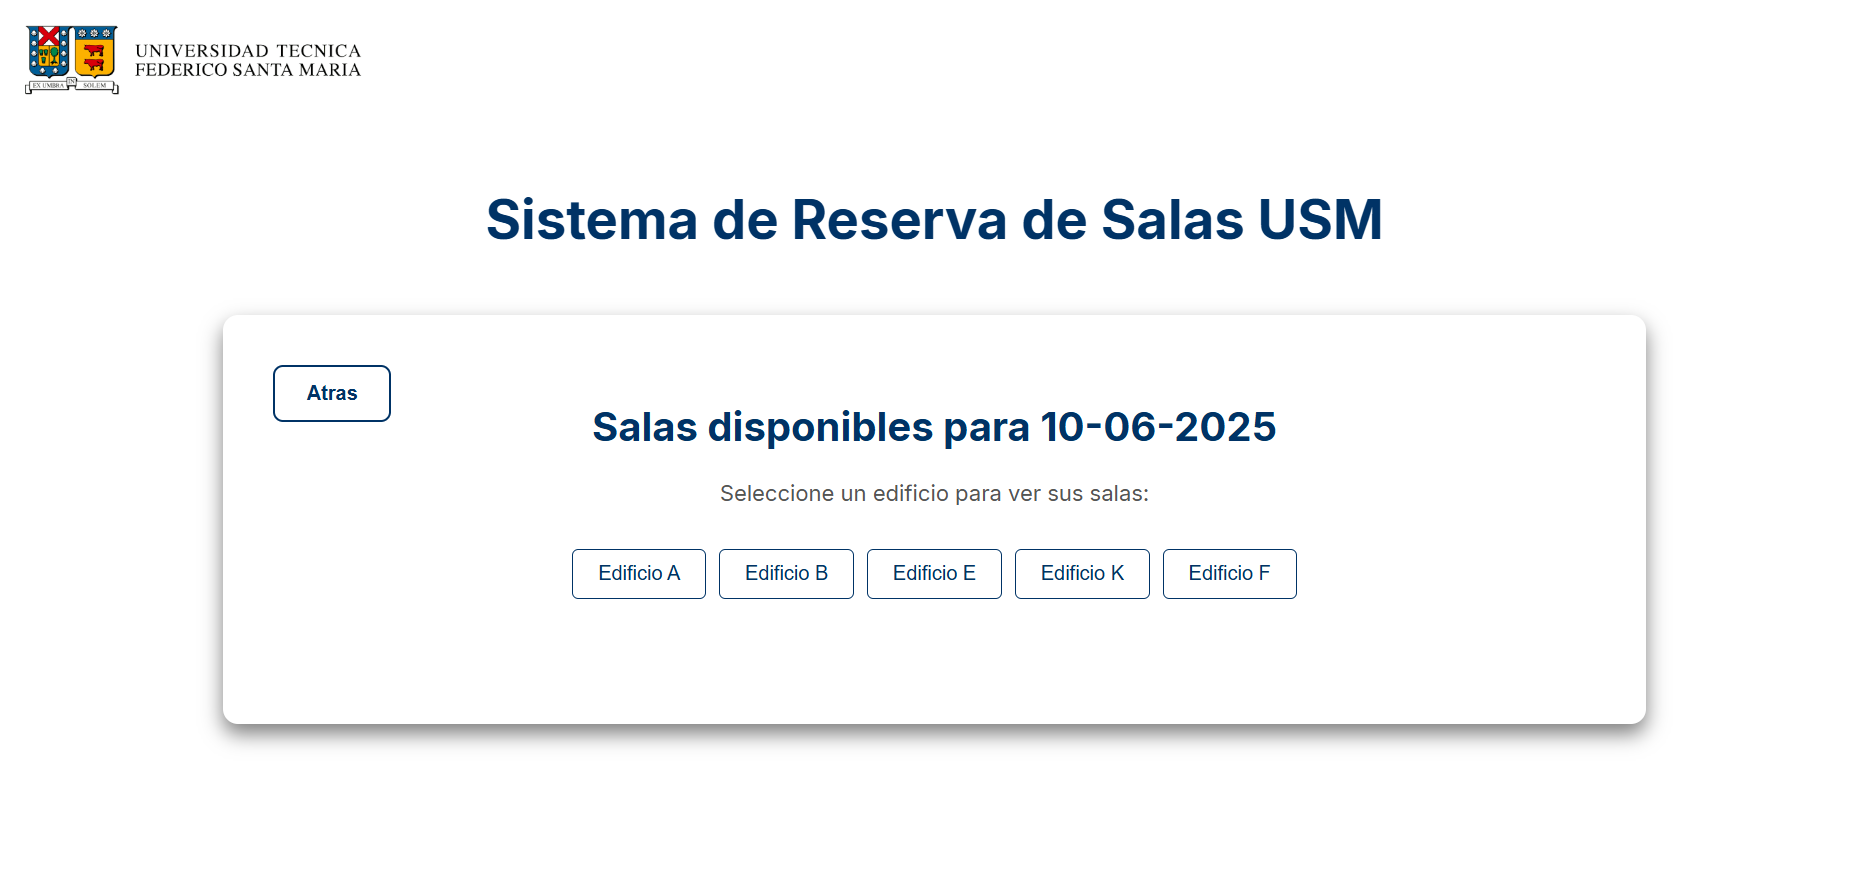
\includegraphics[width=0.8\textwidth]{IMG/ss18.png}
            \end{figure}
            

            \item  \textit{Ver horarios de la Sala K203:}
            \begin{figure}[H] 
                \centering 
                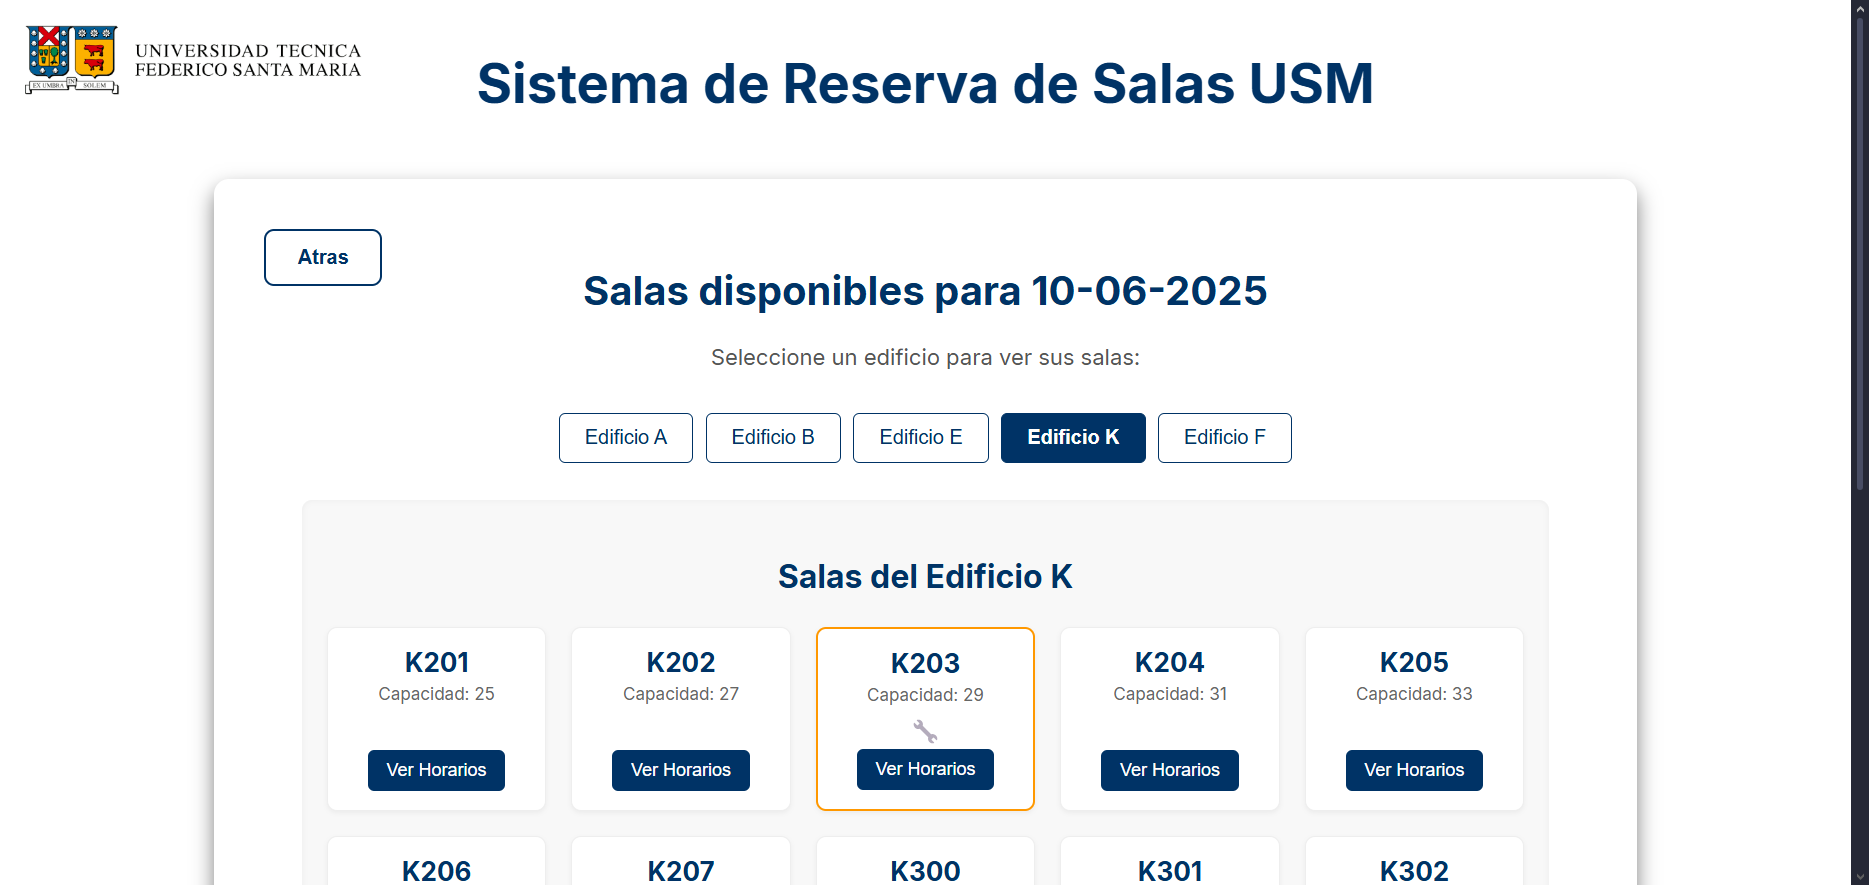
\includegraphics[width=0.8\textwidth]{IMG/ss19.png} 
            \end{figure}

            \item  \textit{Escoger el Bloque 1-2:}
            \begin{figure}[H] 
                \centering 
                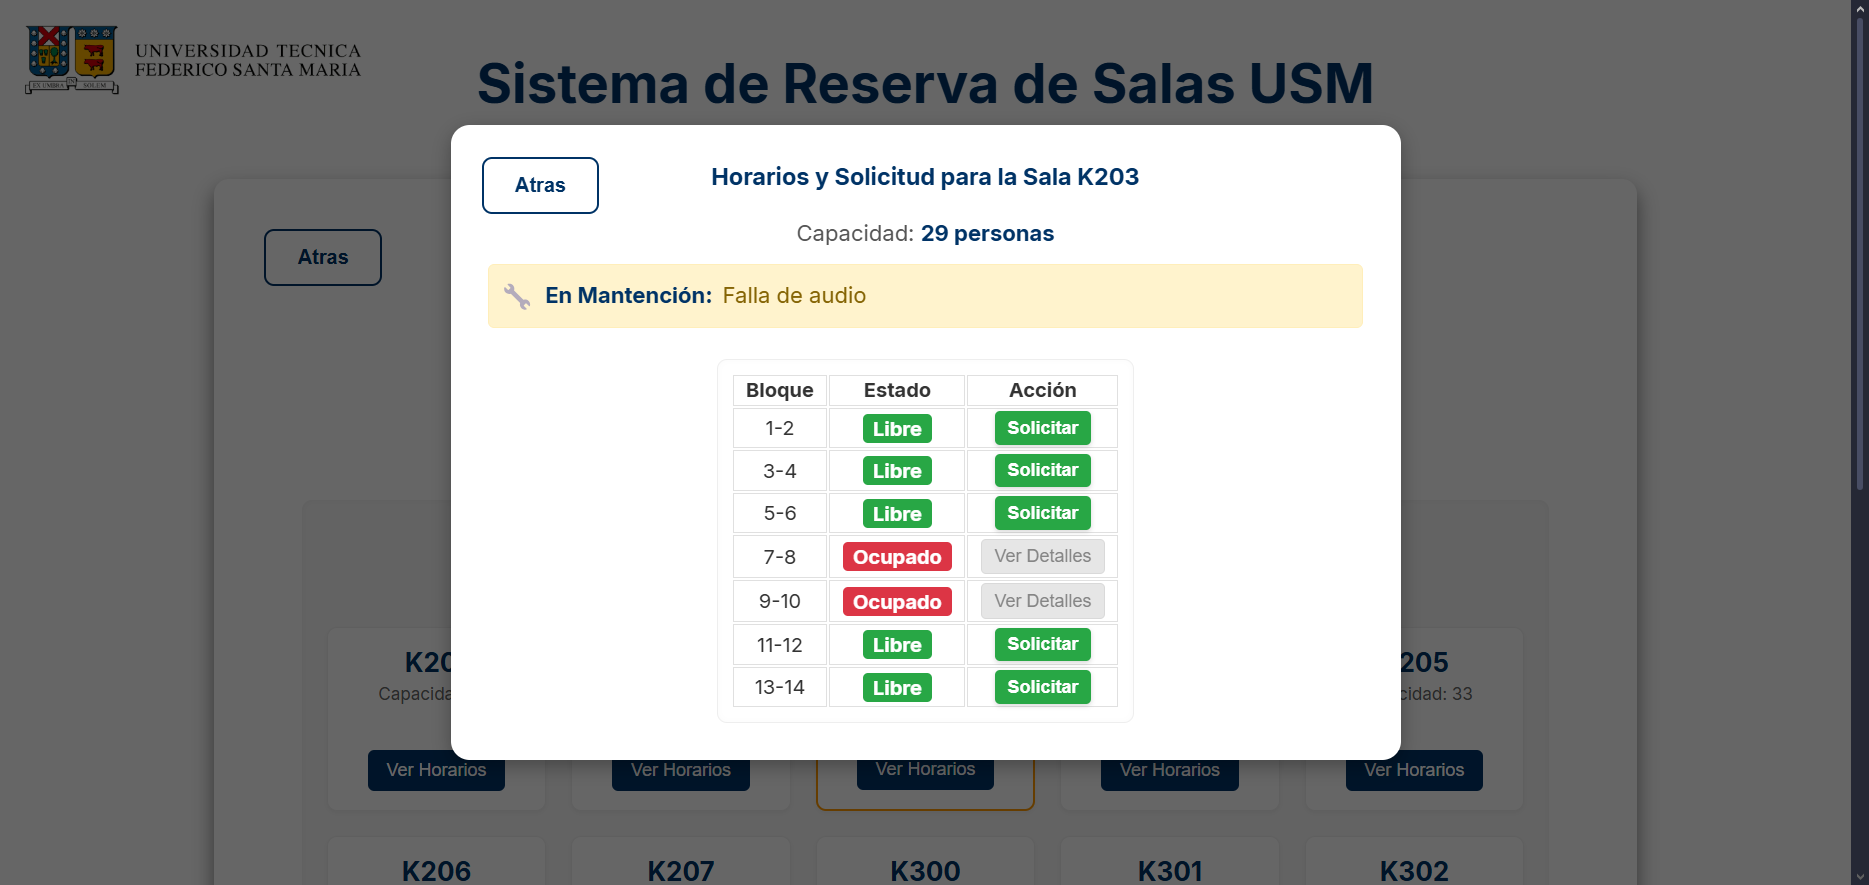
\includegraphics[width=0.8\textwidth]{IMG/ss20.png} 
            \end{figure}

            \newpage
            \item  \textit{Seleccionar cerrar:}
            \begin{figure}[H] 
                \centering 
                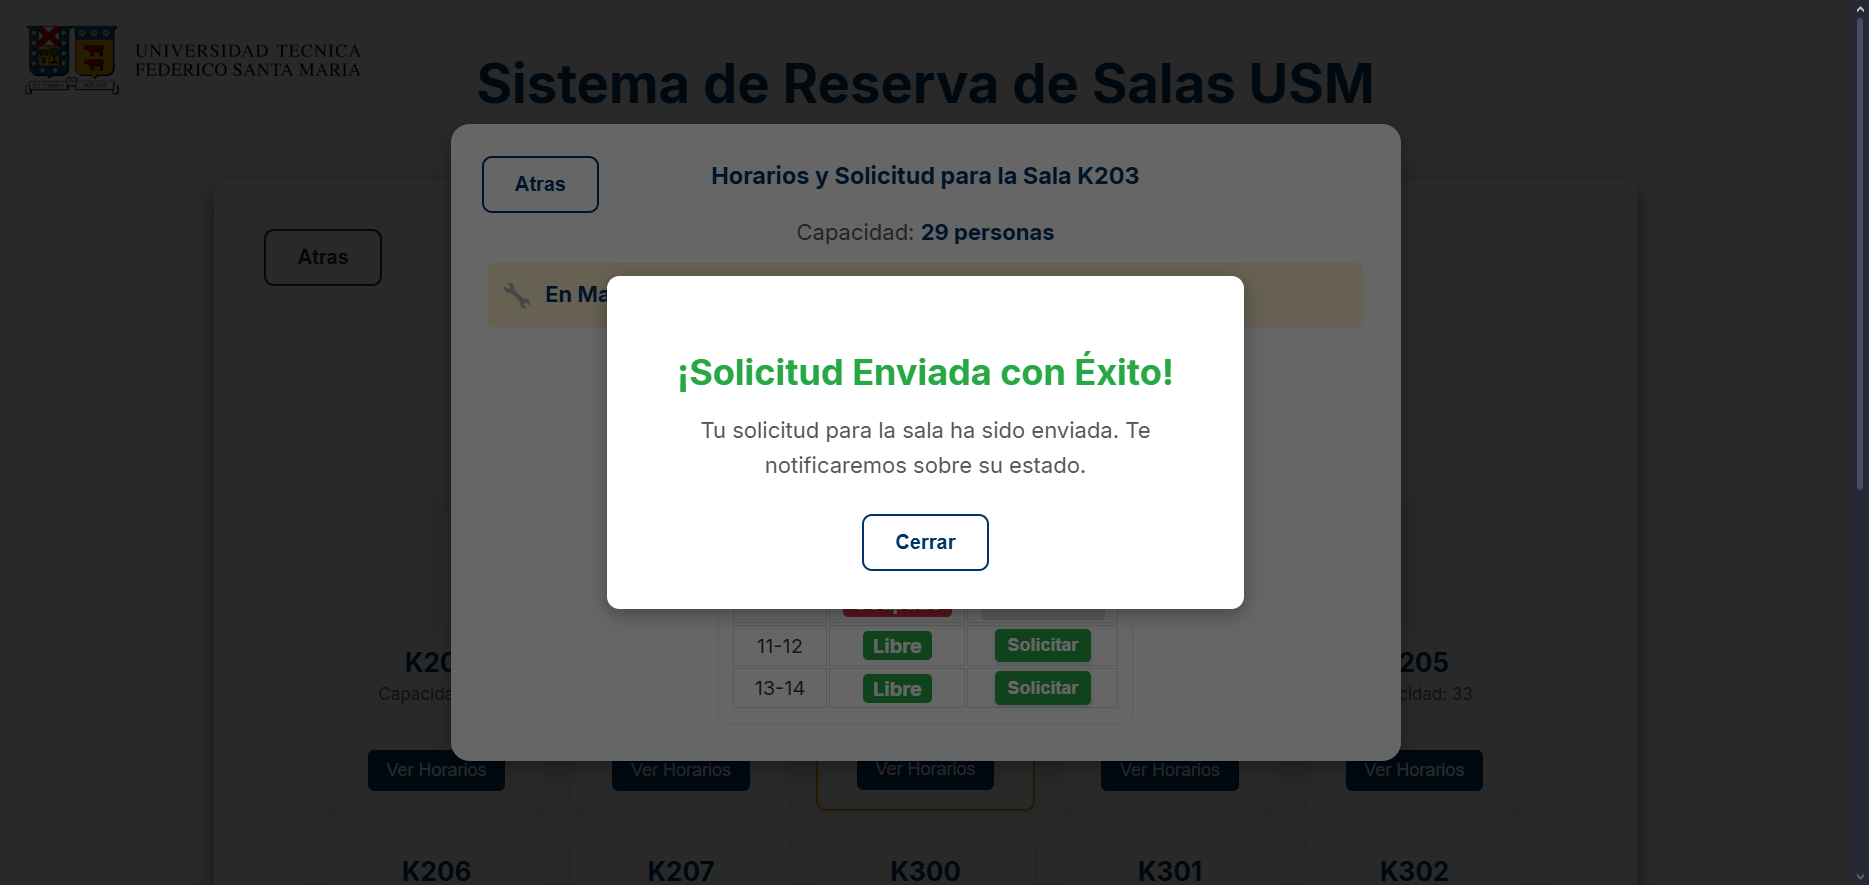
\includegraphics[width=0.8\textwidth]{IMG/ss21.png} 
            \end{figure}

            \item  \textit{Estado final:}
            \begin{figure}[H] 
                \centering 
                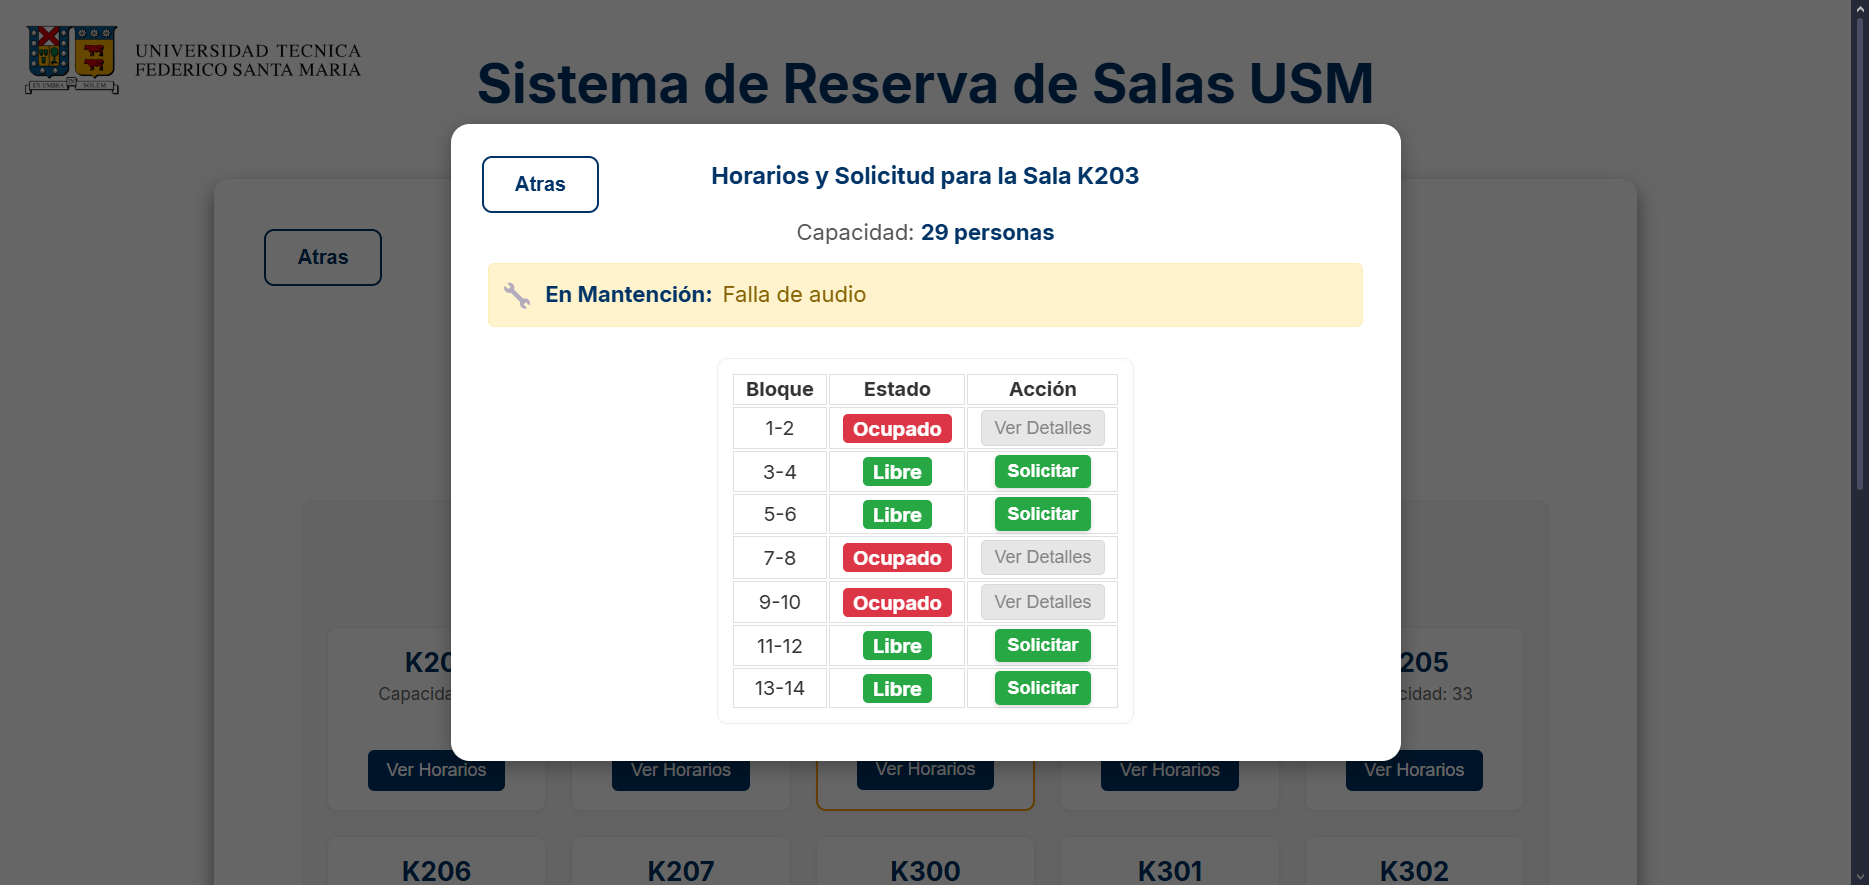
\includegraphics[width=0.8\textwidth]{IMG/ss22.png} 
            \end{figure}
        \end{enumerate}

        \item \textbf{Actualizar estado de la sala Administrador:}
        
        \begin{enumerate}
            \item \textit{Escoger rol administrador:}
            \begin{figure}[H] 
                \centering 
                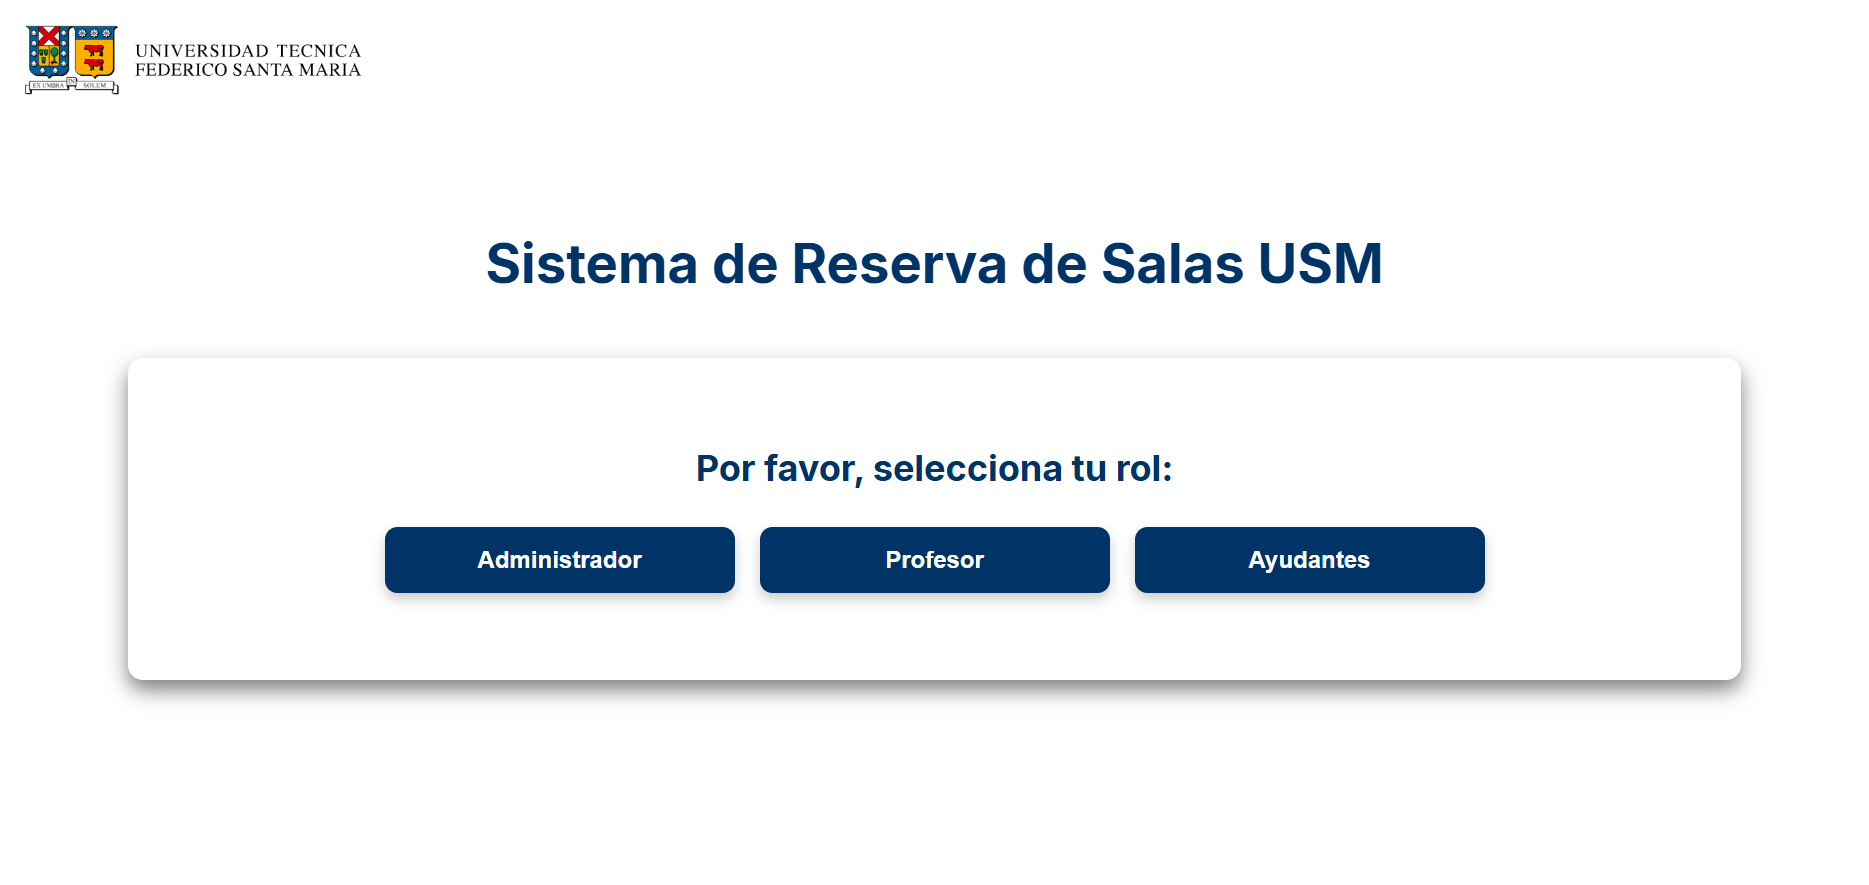
\includegraphics[width=0.8\textwidth]{IMG/ss1.png} 
            \end{figure}

            \newpage
            \item \textit{Escoger el Edificio A:}
            \begin{figure}[H] 
                \centering 
                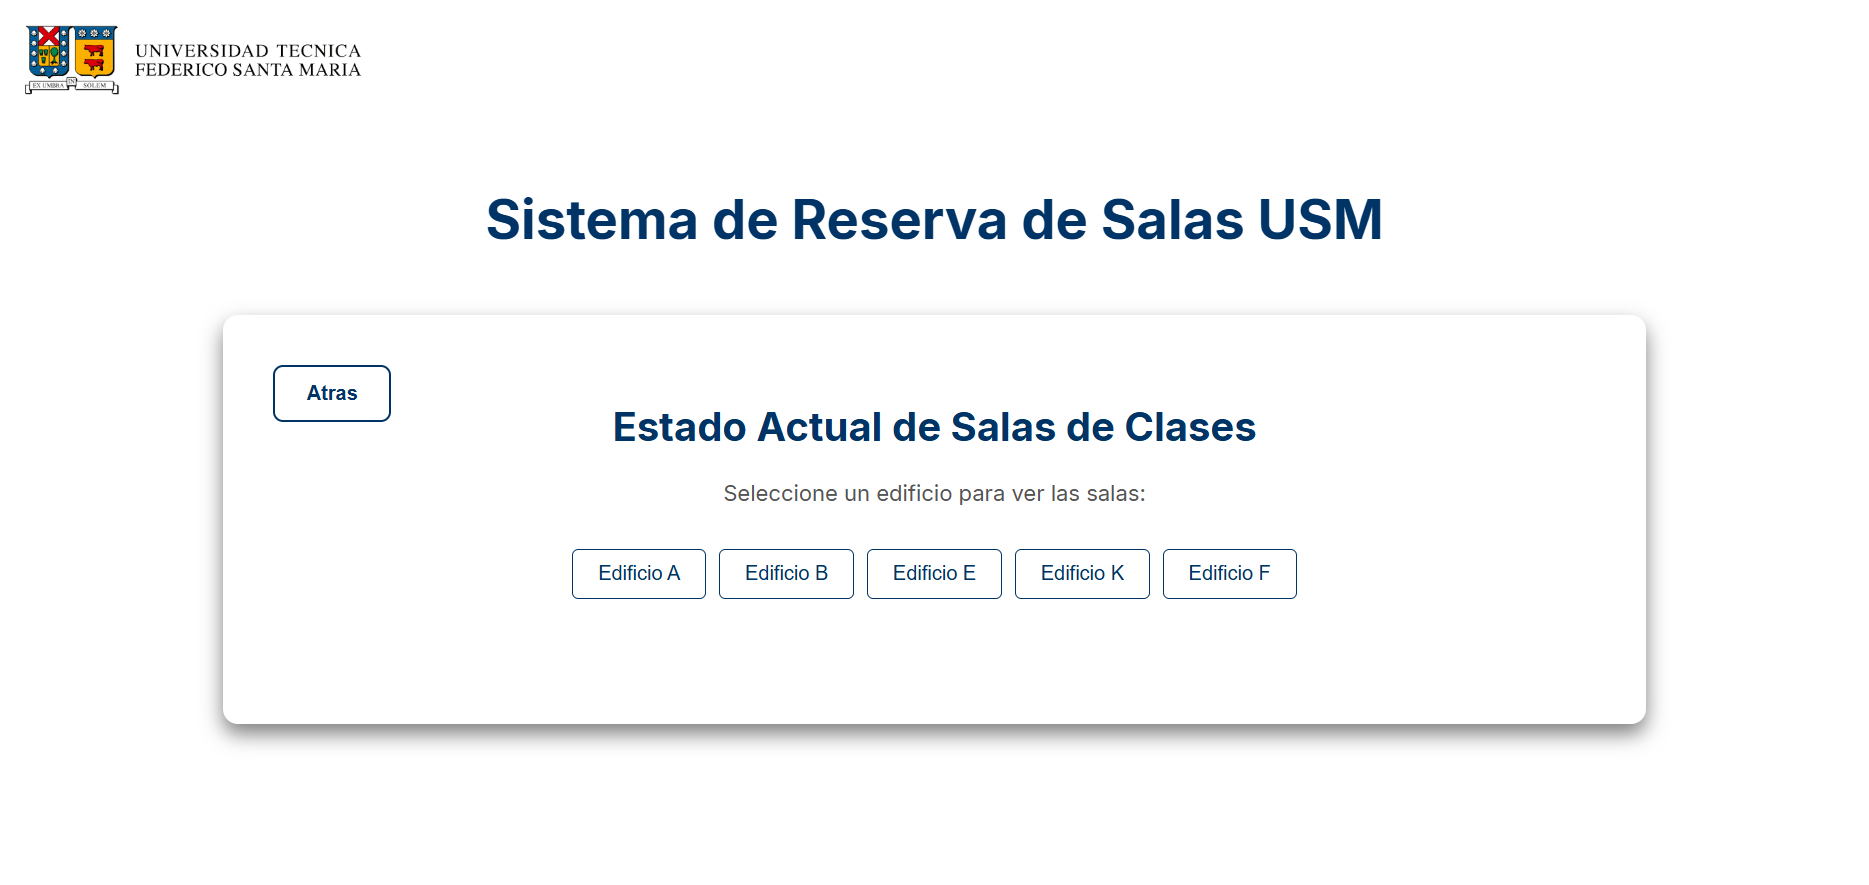
\includegraphics[width=0.8\textwidth]{IMG/ss23.png} 
            \end{figure}

            
            \item \textit{Ver estado de la sala A002:}
            \begin{figure}[H] 
                \centering 
                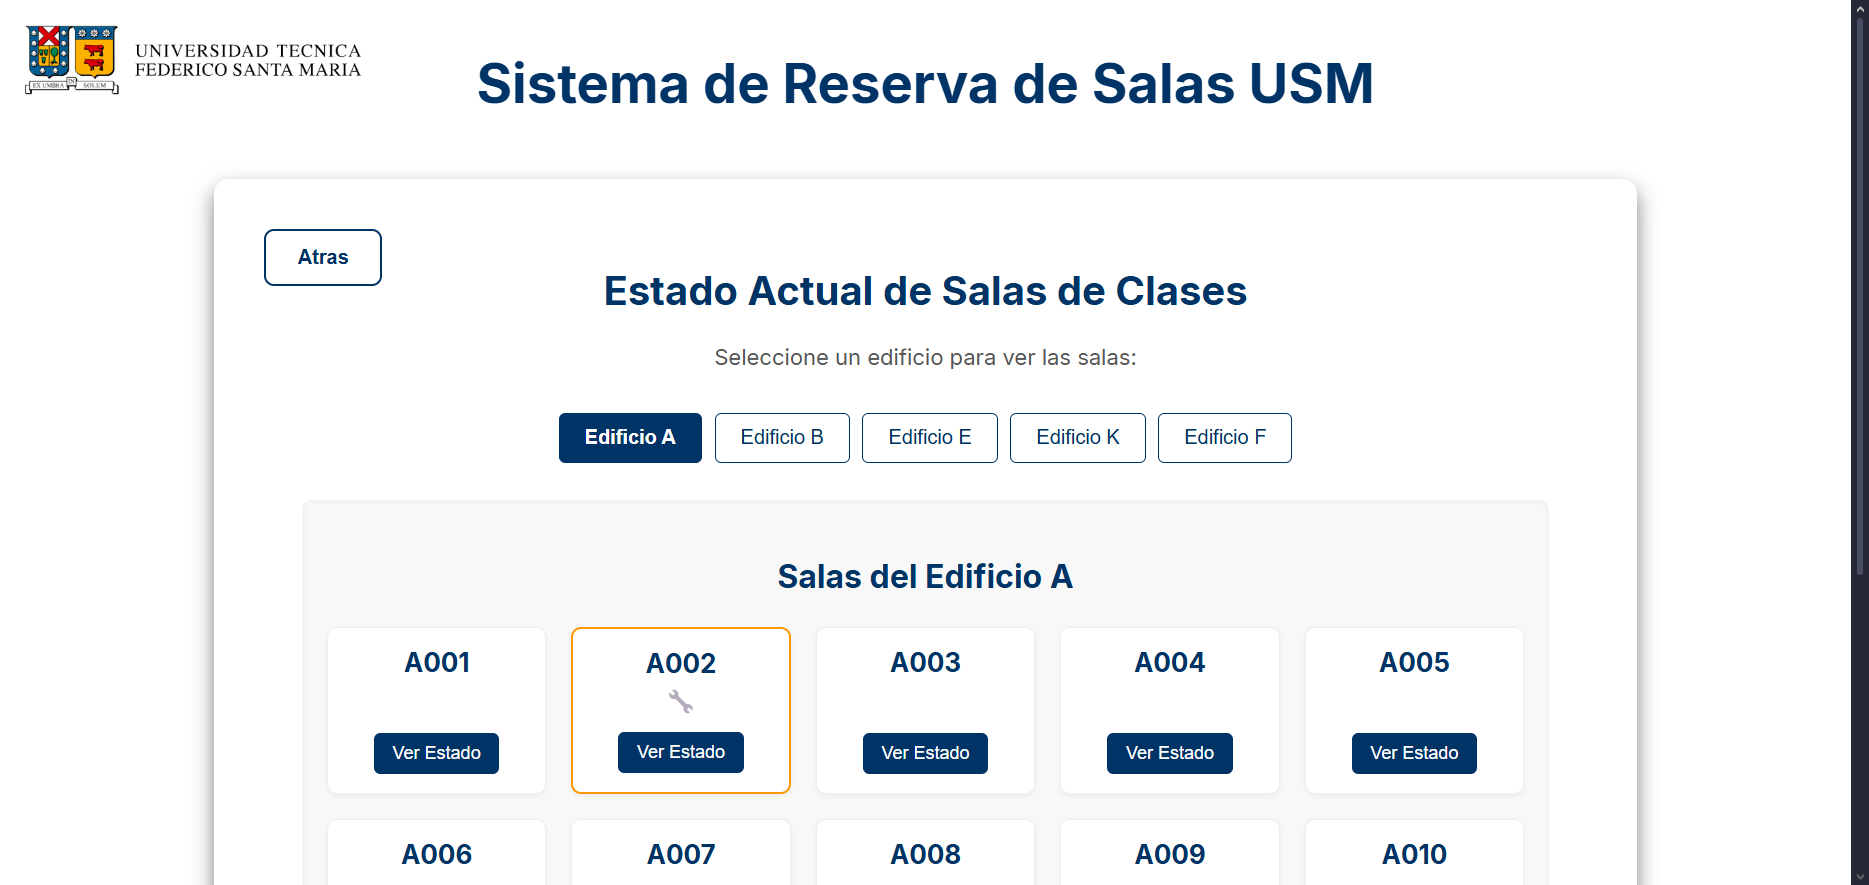
\includegraphics[width=0.8\textwidth]{IMG/ss24.png} 
            \end{figure}

            
            \item \textit{Eliminar el estado En Mantención:}
            \begin{figure}[H] 
                \centering 
                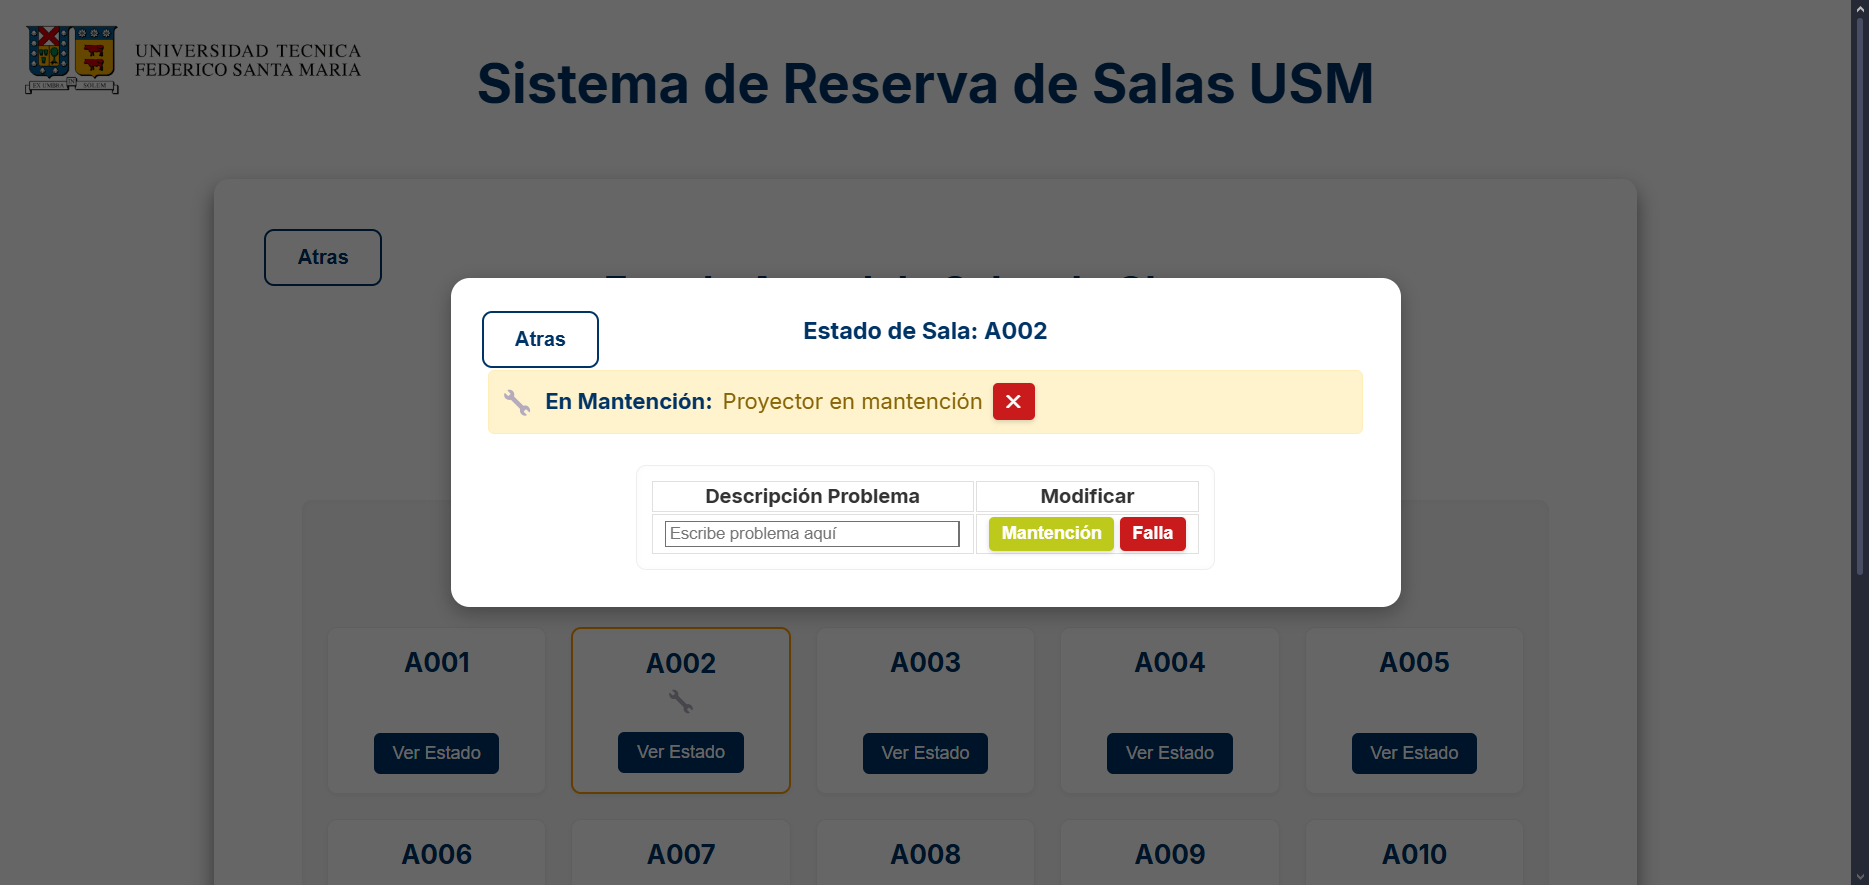
\includegraphics[width=0.8\textwidth]{IMG/ss25.png} 
            \end{figure}

            \newpage
            \item  \textit{Seleccionar cerrar:}
            \begin{figure}[H] 
                \centering 
                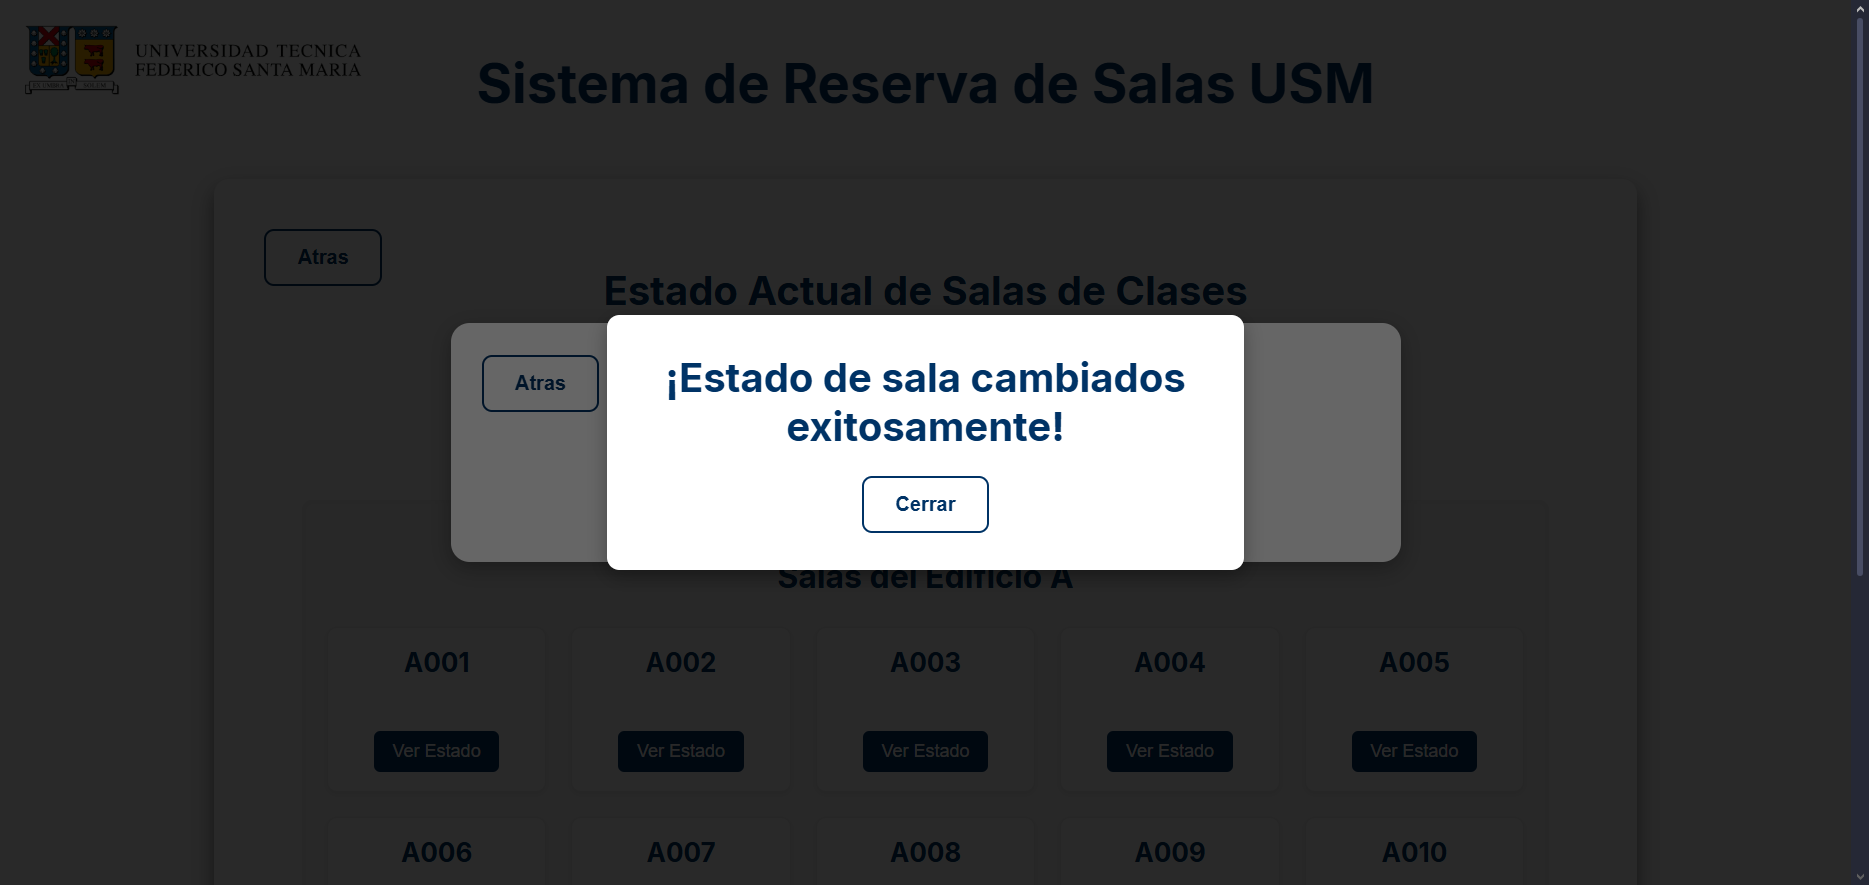
\includegraphics[width=0.8\textwidth]{IMG/ss26.png} 
            \end{figure}
            
            
            \item \textit{Escribir una descripción y seleccionar Falla: }
            \begin{figure}[H] 
                \centering 
                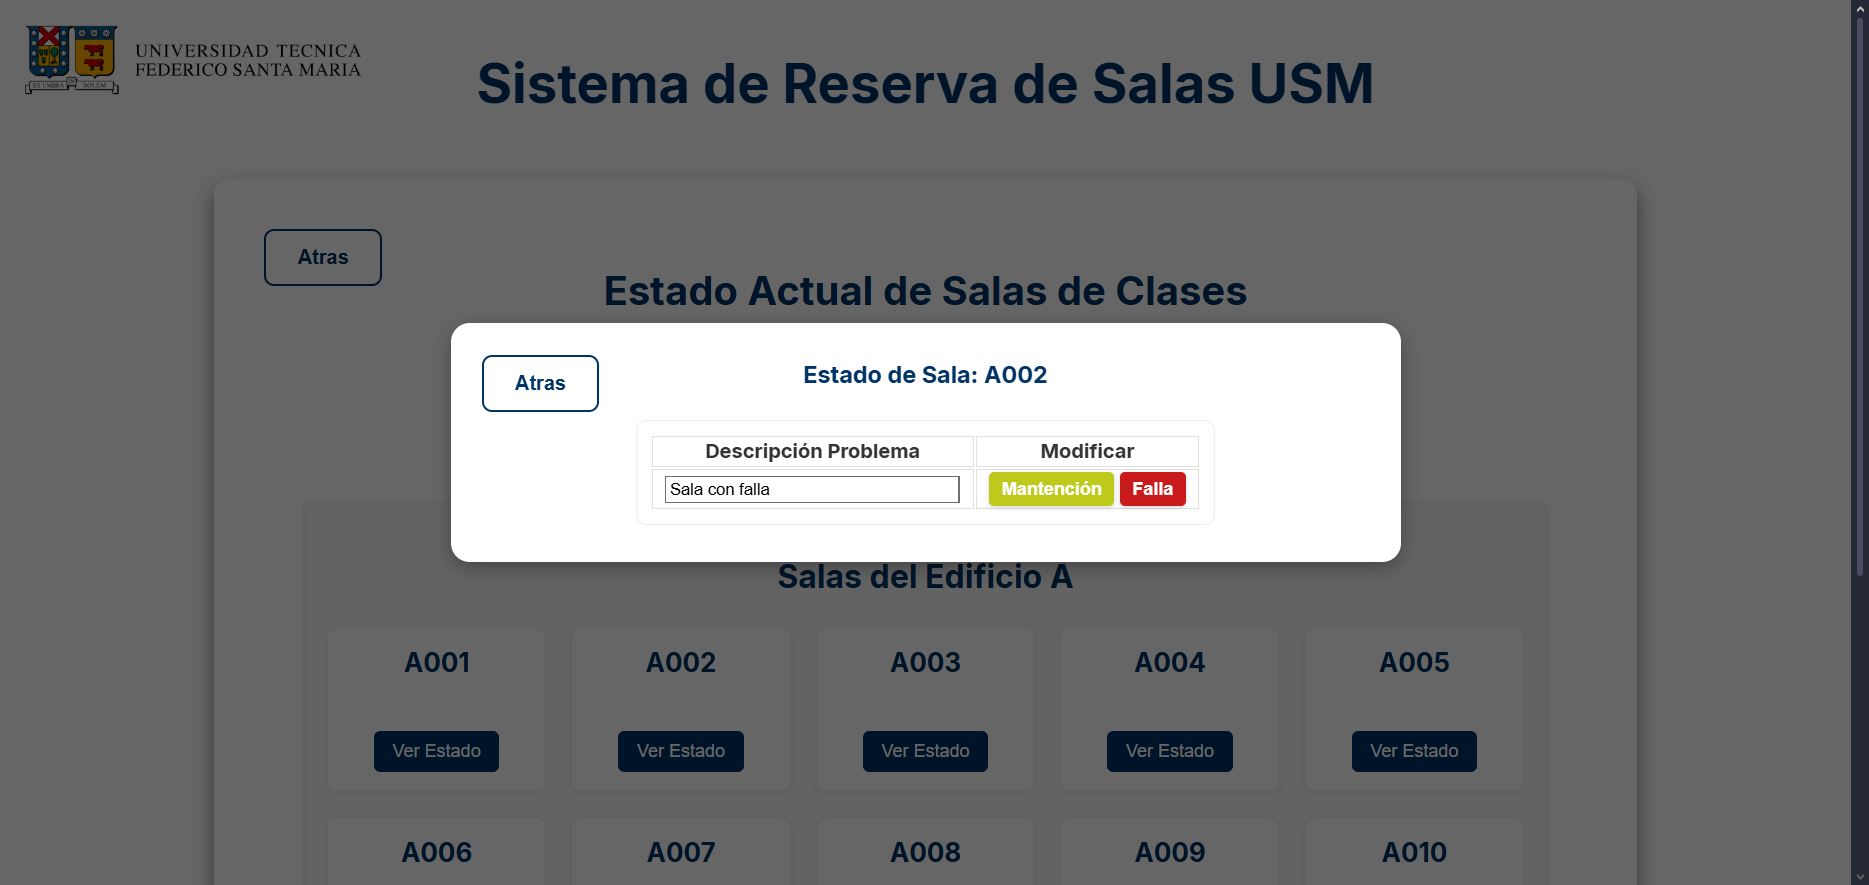
\includegraphics[width=0.8\textwidth]{IMG/ss27.png}
            \end{figure}
            

            \item  \textit{Seleccionar cerrar:}
            \begin{figure}[H] 
                \centering 
                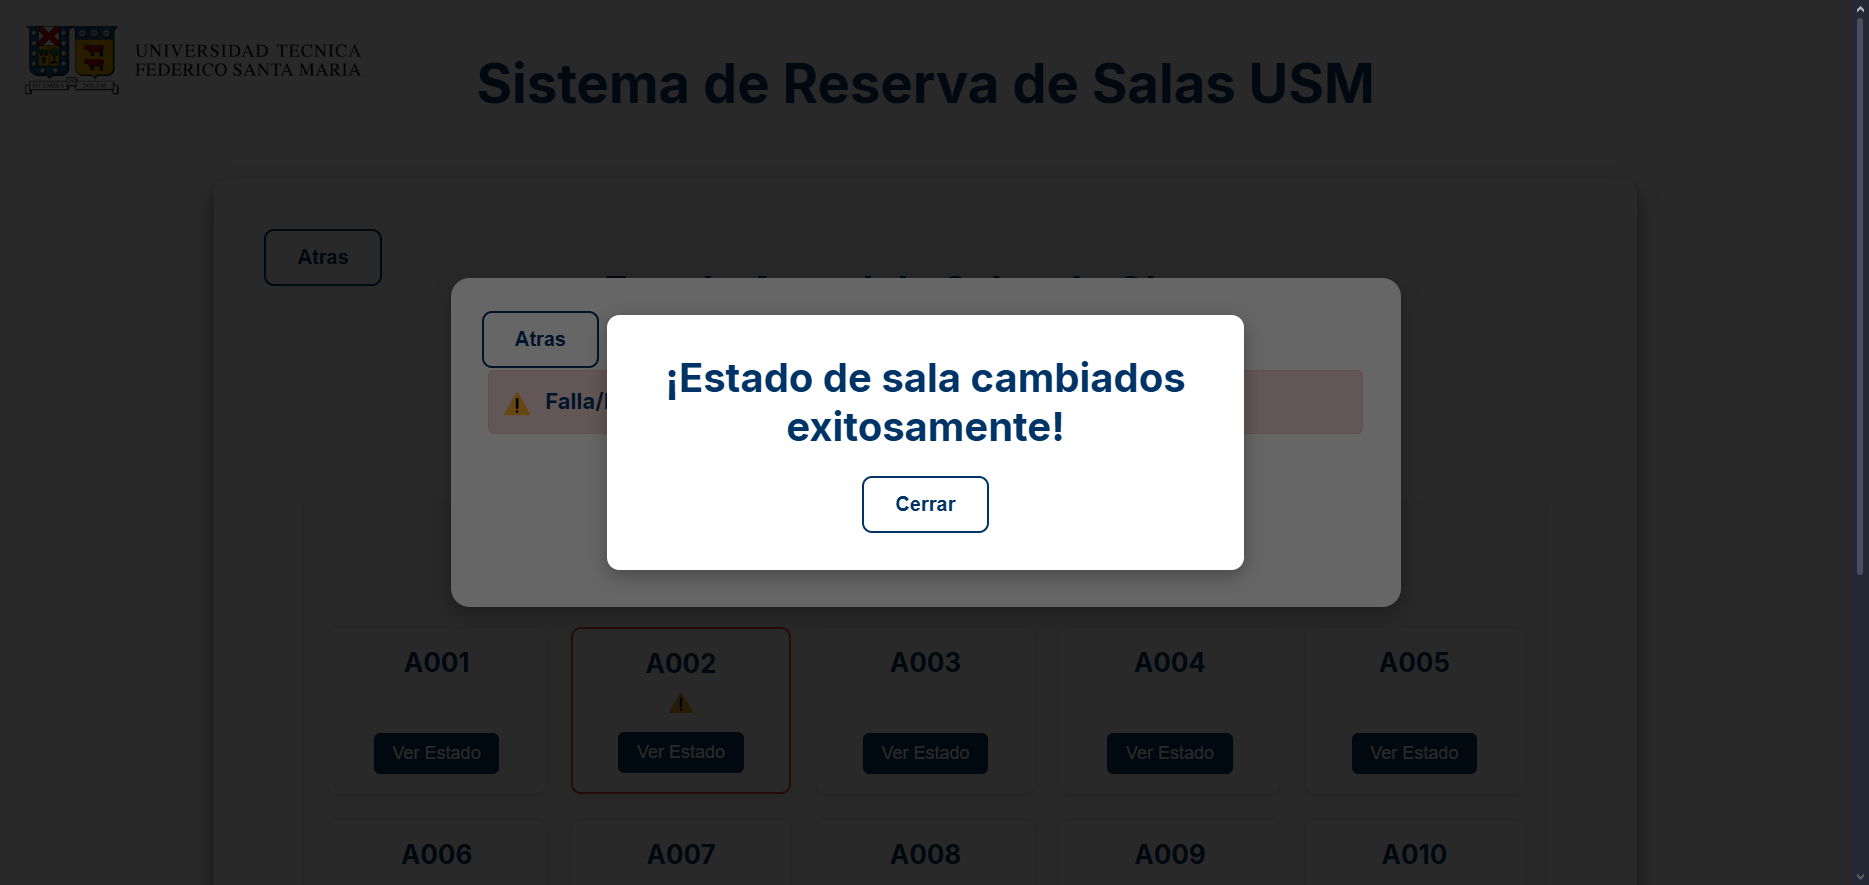
\includegraphics[width=0.8\textwidth]{IMG/ss28.png} 
            \end{figure}

            \newpage
            \item  \textit{Estado final:}
            \begin{figure}[H] 
                \centering 
                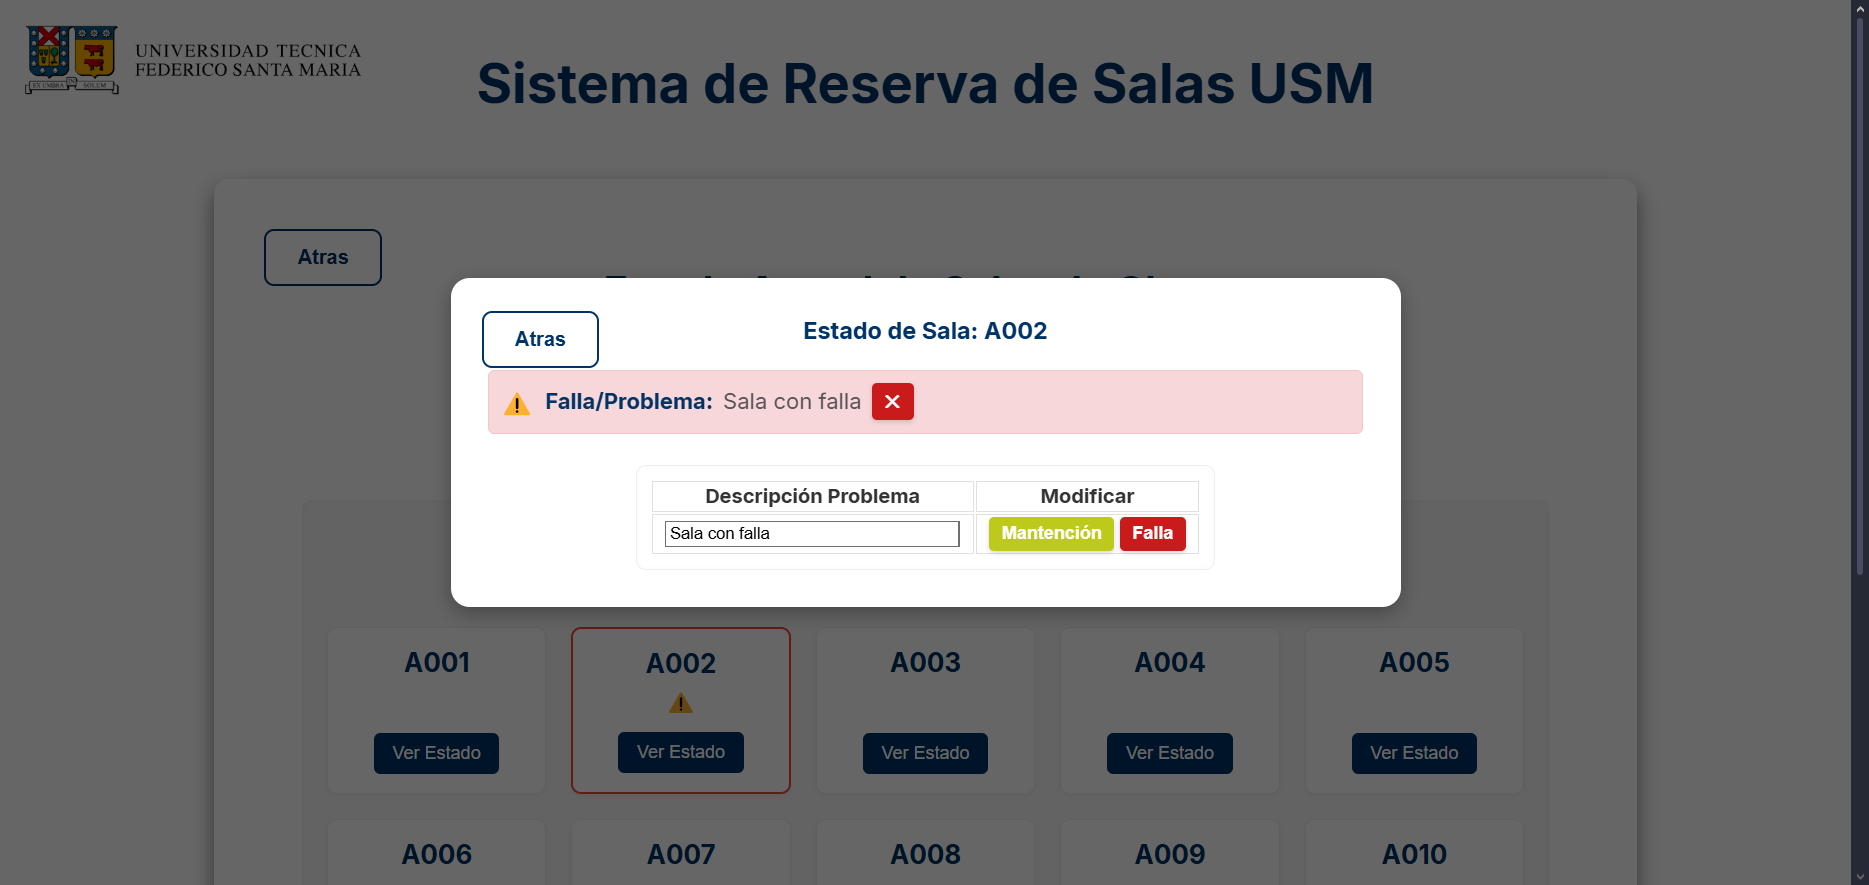
\includegraphics[width=0.8\textwidth]{IMG/ss29.png} 
            \end{figure}

            
        \end{enumerate}
    \end{enumerate}
\end{document}